\documentclass[conference]{IEEEtran}
\IEEEoverridecommandlockouts
% The preceding line is only needed to identify funding in the first footnote. If that is unneeded, please comment it out.
\usepackage{cite}
\usepackage{amsmath,amssymb,amsfonts,amsthm}
\usepackage{algorithm}
\usepackage{algpseudocode}
\usepackage{graphicx}
\usepackage{textcomp}
\usepackage{xcolor}
\usepackage{booktabs}
\usepackage{multirow}
\usepackage{array}
\usepackage[hidelinks]{hyperref}
\renewcommand{\tablename}{Table}

\newtheorem{theorem}{Theorem}
\newtheorem{lemma}{Lemma}
\newtheorem{proposition}{Proposition}
\newtheorem{corollary}{Corollary}
\newtheorem{assumption}{Assumption}
\theoremstyle{definition}
\newtheorem{definition}{Definition}
\theoremstyle{remark}
\newtheorem{remark}{Remark}
\def\BibTeX{{\rm B\kern-.05em{\sc i\kern-.025em b}\kern-.08em
    T\kern-.1667em\lower.7ex\hbox{E}\kern-.125emX}}
\begin{document}

\title{FedOCR: Outlier Client Removal in Federated Learning}

\author{\IEEEauthorblockN{Jianhua Mao\IEEEauthorrefmark{2}, Junqing Yin\IEEEauthorrefmark{2}, Wei Xi\IEEEauthorrefmark{2}, Hanlin Gu\IEEEauthorrefmark{4}, Lixin Fan\IEEEauthorrefmark{4}\textsuperscript{*}}
\IEEEauthorblockA{\IEEEauthorrefmark{2}\textit{National Key Laboratory of Human-Machine Hybrid Augmented Intelligence, Xi'an Jiaotong University, China}\\
\IEEEauthorrefmark{4}\textit{WeBank, China}\\
\{maojianhua, yin\}@stu.xjtu.edu.cn \quad xiwei@xjtu.edu.cn \quad \{ghltsl123, linxi.fan01\}@gmail.com}
\thanks{\textsuperscript{*} Corresponding author: Lixin Fan (linxi.fan01@gmail.com).}
}

\maketitle

\begin{abstract}
Federated learning keeps data on devices, but noisy labels and non-IID data can still hurt training. Many existing defenses clean data during local training at the sample level, which can improve accuracy but often adds extra computation, communication, and privacy-sensitive bookkeeping.

We propose FedOCR, a simple pre-training filter that removes risky clients before federated optimization starts. FedOCR scores each client in two ways: it checks whether the client looks reliable on a small probing set, and it checks whether the remaining clients still cover the target distribution well. Using these signals, FedOCR keeps a client set that is both cleaner and more balanced.

Experiments on MedMNIST, CIFAR-10, and CIFAR-100 show that FedOCR improves robustness under noisy and non-IID settings, reduces the cost of reaching a target accuracy, and can work together with training-stage noisy-label correction. Overall, FedOCR provides a practical front-end step for robust federated learning. The code and supplementary material, including the full theory derivations and additional experimental figures, are available in our GitHub repository: \href{https://github.com/jianhuamao/FedORC}{\textcolor{blue}{https://github.com/jianhuamao/FedORC}}.

\end{abstract}

\begin{IEEEkeywords}
Federated learning, client selection, label noise, Non-IID data, robust learning
\end{IEEEkeywords}

\section{Introduction}

\begin{figure*}[t]
    \centering
    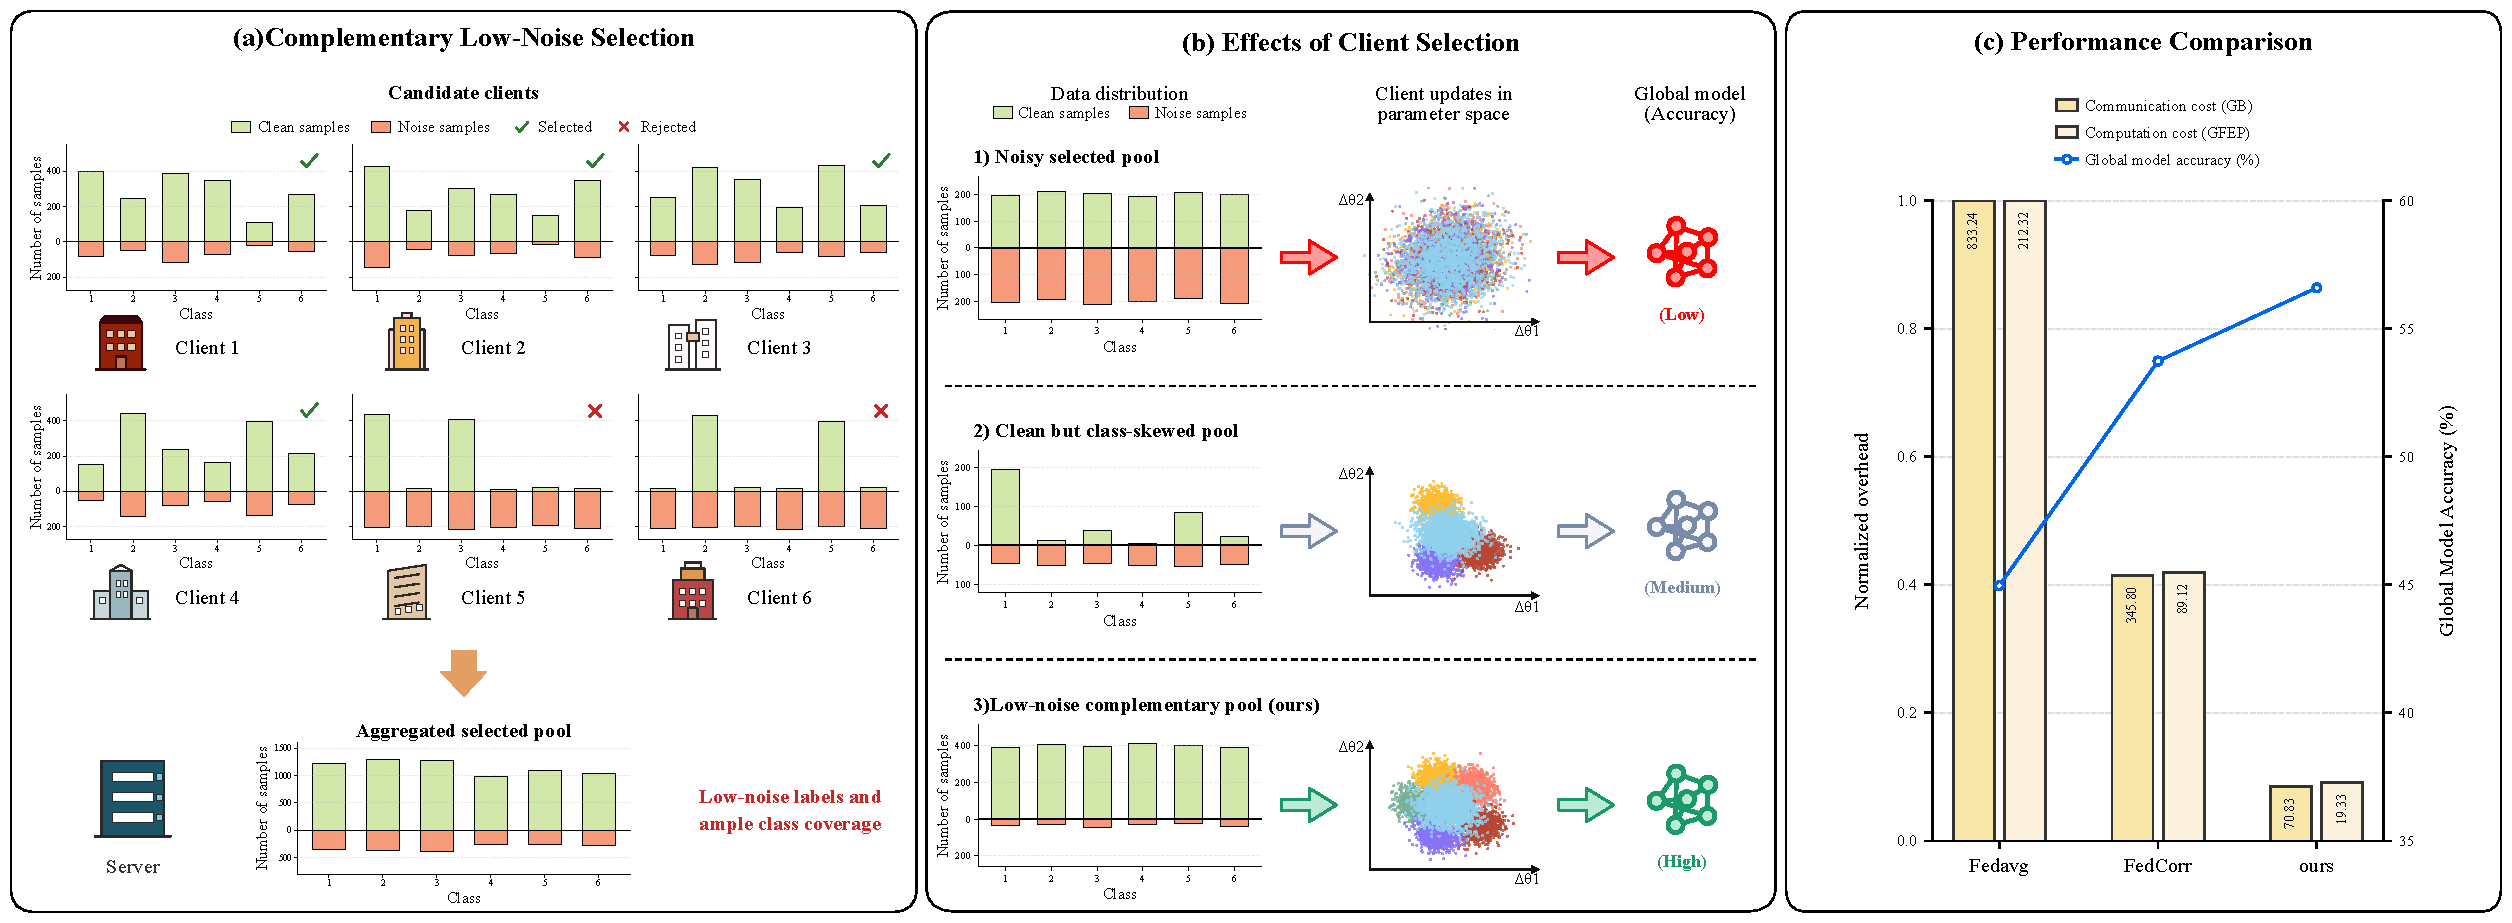
\includegraphics[width=\textwidth]{figure/display_new.pdf}
	\caption{Motivation and effect of FedOCR under heterogeneous noisy-label federated learning. 
		FedOCR performs client-block-level outlier removal before training, retaining a low-risk and complementary participant pool that reduces corrupted updates and improves training efficiency.}
	\label{fig:display}
\end{figure*}
Federated learning (FL) preserves data privacy by keeping data decentralized, yet its practical adoption is hindered by substantial communication and computation overhead. Frequent transmission of large model updates and the limited computational capacity of edge devices are widely recognized as major barriers to real-world deployment~\cite{almanifi2023communication,wen2023survey,le2024practicality,jia2025comst,kairouz2021advances}. This challenge becomes particularly severe in scenarios with heterogeneous client data quality, where label noise and non-IID distributions coexist and often require additional auditing costs per round~\cite{hsu2019measuring,li2021silos,zhu2021survey,liang2023fednoisy}. Thus, a central question arises: how can FL maintain robust performance at low cost under such challenging conditions?

To address robustness under noisy labels, numerous FL methods, commonly referred to as noisy-label FL, have been developed. These approaches typically operate at the sample level during training, using techniques such as sample reweighting, label correction or peer-model filtering to mitigate the impact of corrupted examples~\cite{natarajan2013learning,patrini2017loss,han2018coteaching,northcutt2021confident,tsouvalas2024labeling,xu2022fedcorr,wu2023fednoro,li2024feddiv,hao2025fedcs}. This design is well motivated: label noise occurs at the instance level, and directly handling suspicious samples provides the finest-grained control. From an outlier-processing perspective, these methods can be interpreted as sample-level outlier correction during training.

However, fine-grained correction inevitably incurs non-negligible system costs. When certain clients are persistently noisy or strongly target-mismatched, admitting them in every round is inefficient: the system still spends communication and local computation on these risk-prone clients before their harmful samples are filtered, reweighted, or corrected~\cite{kairouz2021advances,xu2022fedcorr,hao2025fedcs}. FedENLC further makes this burden explicit, showing that label correction can require substantially more computation than standard training~\cite{cho2026fedenlc}. Therefore, sample-level processing alone cannot fully address the efficiency requirement of robust FL.

To achieve both robustness and efficiency, we shift the outlier-removal unit from individual samples to client-side data blocks and perform \textbf{client-level outlier removal before training starts}. This viewpoint is natural in FL: although noise occurs at the sample level, communication, local training, and aggregation are all organized at the client level. Leveraging the block-structured nature of federated data, client-level removal can be equivalently formulated as block-constrained client-level outlier removal (BC-ORS; see definition~\ref{def:sample_block_constrained}).

Our key idea is to exclude high-risk client blocks once before formal federated optimization begins. Because this decision is made at a coarse granularity, it can reduce communication and computation costs throughout subsequent training rounds. Beyond cost savings, client-level outlier removal brings three additional advantages. First, it matches the operational granularity of FL, where the server can admit or reject clients but cannot directly manipulate private samples. Second, it is privacy-compatible, as it does not require the server to request or exchange additional sample-level information~\cite{kairouz2021advances}. Third, it provides robust pre-filtering: by removing risk-prone clients before training, the remaining client pool becomes more reliable, reducing the chance that downstream correction methods are biased by severely corrupted or target-mismatched updates~\cite{xu2022fedcorr,wu2023fednoro,ji2024fedfixer}.

Based on this principle, we propose \textbf{FedOCR}, a reliability- and representativeness-aware framework for pre-training client-level outlier removal. FedOCR operationalizes two core questions: which clients are reliable enough to participate, and whether the retained clients still cover the target-relevant distribution. Specifically, each candidate client first performs a short local adaptation, after which the server evaluates the resulting client model on a server-held probing set. Predictive entropy on the probing set is used to estimate client-block reliability, while KL-based distribution matching evaluates whether the retained client set remains representative of the target-relevant distribution~\cite{northcutt2021confident,guo2017calibration,ben2010theory,lipton2018labelshift,hsu2019measuring,zhu2021survey,zhang2023dpp}.

FedOCR then uses an adaptive greedy rule to integrate reliability and representativeness signals and construct the retained client set. The key point is that the best set size is not fixed blindly: retaining too few clients may lose target coverage, whereas retaining too many can reintroduce accumulated noise. Accordingly, FedOCR aims to retain a client set that contains sufficient clean data while preserving balanced class coverage. As shown in Fig.~\ref{fig:display}(b), such a low-noise and complementary client pool yields the best empirical performance.

Since FedOCR operates before the main FL training stage, it can be flexibly stacked with downstream noisy-label FL methods. Rather than replacing sample-level correction, FedOCR improves the admitted client pool before optimization begins, allowing subsequent robust training methods to operate on a cleaner and more reliable set of clients. Our integration experiments confirm this benefit: combining FedOCR with training-stage methods, including FedCor~\cite{tang2022fedcor}, FedCorr~\cite{xu2022fedcorr}, and FedNoRo~\cite{wu2023fednoro}, improves both accuracy and efficiency compared with using each method alone. Therefore, when higher final accuracy is desired, FedOCR can be coupled with stronger training-stage noisy-label FL methods.

Our main contributions are summarized as follows:
\begin{itemize}
	\item We study robust federated learning from a \textbf{client-block-level outlier-removal perspective}, shifting the denoising unit from individual noisy samples to locality-constrained client data blocks.
	
	\item We propose a \textbf{one-shot pre-training client admission stage} that aligns with the operational structure of FL: the server can admit or reject client blocks without accessing private samples, enabling system-aware risk control before formal optimization.
	
	\item We formulate a \textbf{principled construction of an outlier-removal client set} that jointly accounts for reliability outliers and distributional risks while preserving coverage of target-relevant data.
	
	\item We introduce \textbf{FedOCR}, which integrates probing-set predictive entropy, KL-based distribution matching, and an adaptive greedy selection rule to build the retained client pool. Experiments validate the design, demonstrating lower communication and computation costs at matched target utility and compatibility with training-stage noisy-label FL methods.
\end{itemize}
\section{Related Work}

\paragraph{\textbf{Centralized outlier removal}}
Outlier removal in centralized learning has long focused on instance-level noisy-label filtering and robust training.
Classical approaches correct labels, reweight suspicious samples, or identify clean examples by low loss or high confidence, including loss correction, co-teaching, confident learning, and related noisy-label routines~\cite{natarajan2013noisy,patrini2017loss,han2018coteaching,zhang2021nochange,northcutt2021confident}.
These methods are effective because the learner can directly inspect all samples and, when available, use validation evidence to identify harmful instances.
FedOCR inherits this robustness intuition, but moves the removal decision one level up, to client blocks rather than individual samples.

\paragraph{\textbf{Noisy-label learning in FL}}
Federated learning inherits the same noisy-label problem, but the privacy-preserving and communication-constrained setting makes sample-level correction harder to apply repeatedly~\cite{li2020fedprox,karimireddy2020scaffold,khaled2020convergence,liang2023fednoisy}.
Existing FL methods adapt centralized ideas through label correction, sample reweighting, small-loss selection, peer-model filtering, and local data refinement~\cite{tsouvalas2024labeling,xu2022fedcorr,wu2023fednoro,li2024feddiv,ji2024fedfixer,hao2025fedcs,sivasubramanian2024gradient}.
While effective, these approaches often add extra local computation, confidence tracking, state maintenance, or privacy-sensitive signals, and they typically operate after clients have already been admitted to training~\cite{kairouz2021advances,xu2022fedcorr,hao2025fedcs}.
FedOCR targets an earlier stage: it screens client blocks before training so that downstream methods can work on a cleaner participant pool.

\paragraph{\textbf{Client-level dynamic outlier removal}}
A separate line of work studies client selection to improve FL efficiency and convergence under communication and resource constraints~\cite{fu2023client,almanifi2023communication,le2024practicality,jia2025comst}.
Representative methods choose clients by estimated utility, loss, gradient correlation, diversity, or cluster-level informativeness~\cite{lai2021oort,cho2022power,tang2022fedcor,zhang2023dpp,ACFL}.
Most of these methods are round-wise schedulers: they ask which clients are useful for the current communication round, not whether a client should remain in the pool at all.
FedOCR extends this client-level pruning view by jointly considering reliability and subset-level representativeness.
Because the server cannot inspect raw data directly, these criteria are realized through privacy-compatible probing signals, namely probing-set predictive entropy and KL-based probing distribution matching.

\section{Theoretical Analysis}
\label{sec:theoretical_analysis}

We study \emph{pre-training outlier removal} for federated learning (FL) from a client-level perspective. 
Our goal is to select a subset of training samples that minimizes the target risk, while respecting FL constraints that isolate samples into client-specific blocks.

\subsection{Problem Setup}
\label{subsec:problem_setup}
Let $P_T$ denote the target distribution, and $h\in\mathcal{H}$ any hypothesis with target risk
\begin{equation}
	\epsilon_T(h) = \mathbb{E}_{(x,y)\sim P_T}[\ell(h(x),y)].
\end{equation}
\begin{assumption}[Existence of risk-prone data]
	\label{assump:risk_prone_data}
	The candidate training collection $D$ contains a non-empty subset of risk-prone samples
	$D_{\mathrm{risk}}\subset D$.
	Samples in $D_{\mathrm{risk}}$ may contain persistent risks, such as corrupted labels or target-mismatched examples, which can harm the target model if they are retained for training.
\end{assumption}
\begin{definition}[Sample-level outlier-removal set (ORS)]
	\label{def:sample_golden_set}
	In a centralized setting where all training samples $D$ are accessible, the optimal retained sample subset is
	\begin{equation}
		S_{\mathrm{ORS}} \in \arg\min_{\emptyset\neq 
		S\subseteq D} \epsilon_T(h_S),
	\end{equation}
	where $h_S$ is trained on subset $S$. This defines the \emph{sample-level outlier-removal set}.
\end{definition}

\begin{definition}[Block-constrained ORS (BC-ORS) under FL]
	\label{def:sample_block_constrained}
	In FL, samples are partitioned into client blocks $D=\bigsqcup_{i=1}^N D_i$, $D_i$ donates private data on client $i$.
	For a given subset of sample blocks $S^\star=\bigsqcup_{i=1}^M D_i$, and $M\subseteq\{1,\dots,N\}$, define the retained sample set The \emph{sample-block-constrained ORS} is
	\begin{equation}
		S^\star_{\mathrm{BC-ORS}} \in \arg\min_{\emptyset\neq S^\star \subseteq \{1,\dots,N\}} \epsilon_T(h_{S^\star}),
	\end{equation}
	where $h_{S^\star}$ is trained on the retained samples in $S^\star$. 
	Compared to centralized ORS, the only constraint is that samples cannot be selected individually; instead, entire client blocks are retained or discarded.
\end{definition}

\begin{remark}[ORS versus BC-ORS]
\label{rem:ORS_vs_BC-ORS}
ORS is the sample-level oracle benchmark and BC-ORS is the FL-constrained counterpart. Therefore, BC-ORS is generally slightly suboptimal to ORS in target accuracy. We nevertheless prefer BC-ORS in FL because privacy and locality constraints rule out sample-level auditing, and because finding BC-ORS is orders of magnitude more efficient in communication and computation, as illustrated in Fig.~\ref{fig:display}(c) and Section~\ref{sec:experiment}.
\end{remark}

\subsection{A Unified Risk View of Client-Block Outlier Removal}
\label{subsec:risk_view}

We now formalize why pre-training client-level outlier removal is justified.
Since FL cannot realize sample-level ORS, the key question is whether a retained client-block set $S$ lowers the target-risk upper bound.
In this section, our analysis shows that two factors matter: unreliable clients can inject noisy supervision, and an imbalanced retained pool can drift away from the target distribution~\cite{hsu2019measuring,li2021silos,zhu2021survey}.

\begin{assumption}[Bounded loss]
\label{assump:bounded_loss}
The loss function is bounded:
\begin{equation}
0\le \ell(h(x),y)\le 1,
\qquad
\forall h\in\mathcal{H},\ (x,y)\in\mathcal{X}\times\mathcal{Y}.
\end{equation}
\end{assumption}

\begin{assumption}[Label-shift-dominated heterogeneity]
\label{assump:label_shift}
For every clean client distribution $\mu_i$ and the target distribution $P_T$, the class-conditional distribution is shared:
\begin{equation}
\mu_i(x,y)=p(x\mid y)q_i(y),
\qquad
P_T(x,y)=p(x\mid y)q_T(y),
\end{equation}
where $q_i\in\Delta^{K-1}$ is the clean label prior of client $i$, and $q_T\in\Delta^{K-1}$ is the target label prior.
\end{assumption}

Assumption~\ref{assump:label_shift} focuses on label-prior heterogeneity, where clients differ mainly in class proportions rather than in class-conditional feature distributions~\cite{lipton2018labelshift,hsu2019measuring}.
Thus, the theoretical bound characterizes a label-shift-dominated case of Non-IID FL.

For a selected subset $S$, define its clean mixture label prior as
\begin{equation}
\bar q_S
=
\sum_{i\in S}w_i(S)q_i,
\qquad
w_i(S)=\frac{n_i}{\sum_{j\in S}n_j}.
\end{equation}
Under Assumption~\ref{assump:label_shift}, the clean selected-client mixture can be written as
\begin{equation}
P_S^c(x,y)=p(x\mid y)\bar q_S(y).
\end{equation}

\begin{assumption}[Label-only noise]
\label{assump:label_only_noise}
For any selected subset $S$, the clean selected-client mixture $P_S^c(X,Y)$ and the noisy selected-client mixture $P_S^n(X,\widetilde Y)$ share the same input marginal:
\begin{equation}
P_S^c(X)=P_S^n(X).
\end{equation}
That is, label noise only corrupts the clean label $Y$ into the observed label $\widetilde Y$.
\end{assumption}
This label-only corruption model follows the standard noisy-label learning setting, including symmetric label noise used in many robustness studies~\cite{natarajan2013learning,patrini2017loss,liang2023fednoisy}.

Define the posterior label-noise discrepancy as
\begin{equation}
\label{eq:posterior_noise_discrepancy}
\xi_{\mathrm{noise}}(S)
=
\mathbb{E}_{x\sim P_S^X}
\left[
\sum_{c=1}^{K}
\left|
P_S^c(Y=c\mid x)
-
P_S^n(\widetilde Y=c\mid x)
\right|
\right].
\end{equation}

\begin{lemma}[Posterior-noise decomposition]
\label{lem:noise_bridge}
Under Assumptions~\ref{assump:bounded_loss} and~\ref{assump:label_only_noise}, 
for any $h\in\mathcal H$ and any selected subset $S$, let
$\epsilon_S^c(h)$ and $\epsilon_S^n(h)$ denote the clean and noisy risks on $S$, respectively. Then,
\begin{equation}
\label{eq:clean_noisy_bridge}
\left|
\epsilon_S^c(h)-\epsilon_S^n(h)
\right|
\le
\xi_{\mathrm{noise}}(S).
\end{equation}
Consequently,
\begin{equation}
\epsilon_S^c(h)
\le
\epsilon_S^n(h)
+
\xi_{\mathrm{noise}}(S).
\end{equation}
\end{lemma}

This lemma should be interpreted as a risk decomposition showing how label corruption enters the target-risk bound.
It does not claim that the posterior discrepancy in Eq.~\eqref{eq:posterior_noise_discrepancy} is directly observable by the server.

\begin{lemma}[Clean target-transfer under label shift]
\label{lem:label_shift_transfer}
Under Assumptions~\ref{assump:bounded_loss} and~\ref{assump:label_shift}, for any $h\in\mathcal{H}$ and any selected subset $S$,
\begin{equation}
\label{eq:clean_transfer}
\epsilon_T(h)
\le
\epsilon_S^c(h)
+
\frac{1}{2}\|\bar q_S-q_T\|_1.
\end{equation}
\end{lemma}



\begin{theorem}[Unified client-block risk bound]
\label{thm:main_bound}
Combining Lemma~\ref{lem:label_shift_transfer} with Lemma~\ref{lem:noise_bridge}, we obtain that, for any selected subset $S$ and any $h\in\mathcal{H}$,
\begin{equation}
\label{eq:main_bound}
\epsilon_T(h)
\le
\epsilon_S^n(h)
+
\xi_{\mathrm{noise}}(S)
+
\frac{1}{2}\|\bar q_S-q_T\|_1.
\end{equation}
\end{theorem}

Theorem~\ref{thm:main_bound} identifies two population-level factors that should be controlled by a retained client-block set: the noise-contamination term $\xi_{\mathrm{noise}}(S)$ and the distribution-mismatch term $\|\bar q_S-q_T\|_1$.
Thus, BC-ORS is not merely a heuristic pre-processing step; changing the retained block set $S$ directly changes the upper bound on the target risk, consistent with domain-adaptation views that link target risk to source risk and distribution discrepancy~\cite{bendavid2006analysis,ben2010theory}.
At the same time, these population quantities are not directly visible to the server before training.
The next subsection therefore turns the bound into an operational probing-consistency statement: FedOCR optimizes observable probing-set surrogates, while the approximation gap between these surrogates and the population quantities is kept explicit through residual terms.

\subsection{From Population Bound to probing Outlier-Removal Surrogates}
\label{subsec:probing_theory}

The bound in Theorem~\ref{thm:main_bound} lives at the population level, 
but quantities in bound cannot be inspected by the server under the privacy and locality constraints of FL~\cite{kairouz2021advances}.
FedOCR therefore instantiates the two risk factors through probing-set probing statistics.This step is not treated as an exact substitution.
Instead, we formulate a residualized probing bound that separates the observable entropy--KL surrogate from the residual terms induced by probing mismatch.
The resulting theory gives a conditional but explicit bridge: when the probing set is target-relevant and the short-adapted client models provide informative uncertainty and class-coverage signatures, optimizing the probing objective is aligned with reducing the population risk factors identified above.
\begin{figure*}[t]
	\centering
	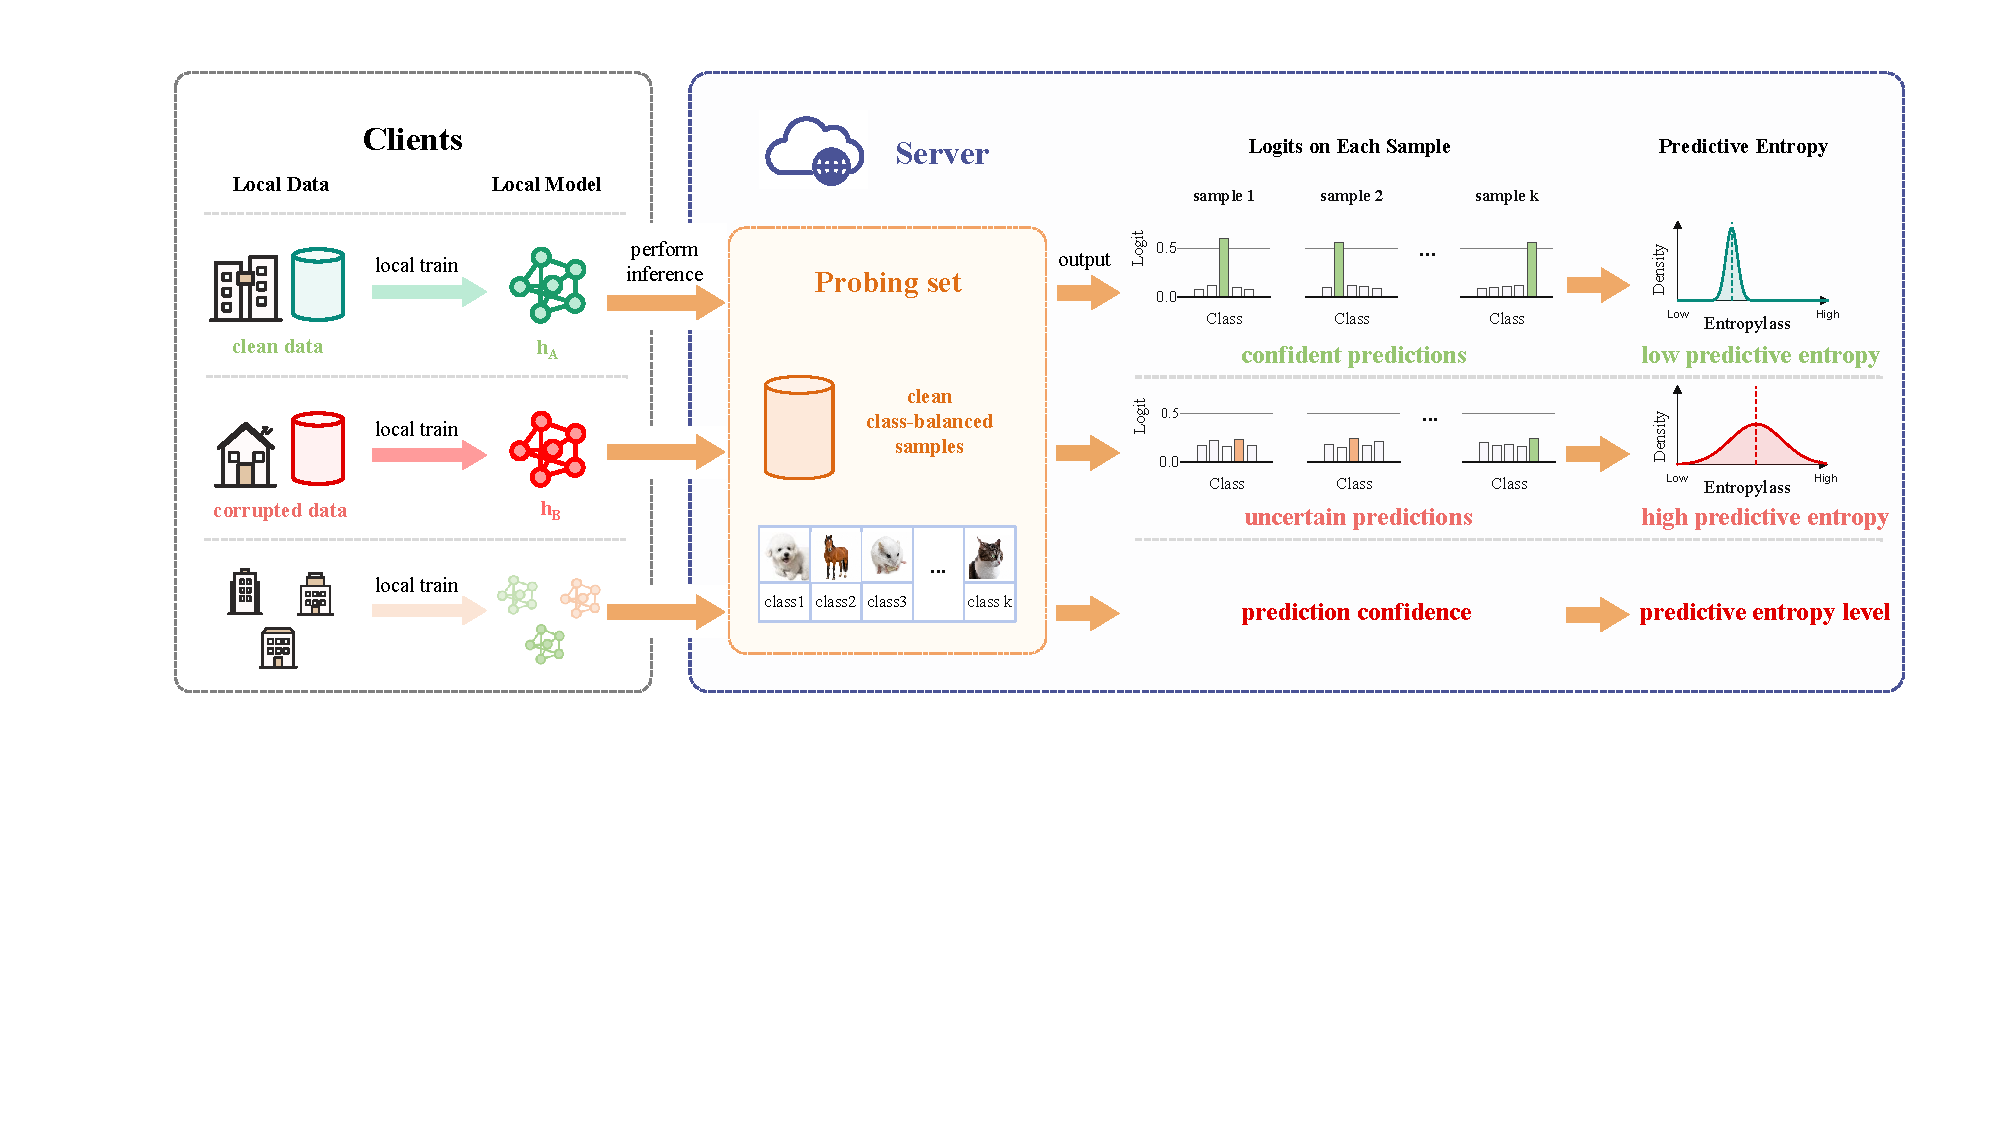
\includegraphics[width=\textwidth]{figure/entropy_prediction_diagram.pdf}
	\caption{Illustration of probing-set predictive entropy for client-block reliability estimation. Each candidate client adapts on its private block, and the server scores the adapted model on clean probing inputs without using probing-set labels.}
	\label{fig:entropy_illustration}
\end{figure*}

\begin{figure}
    \centering
    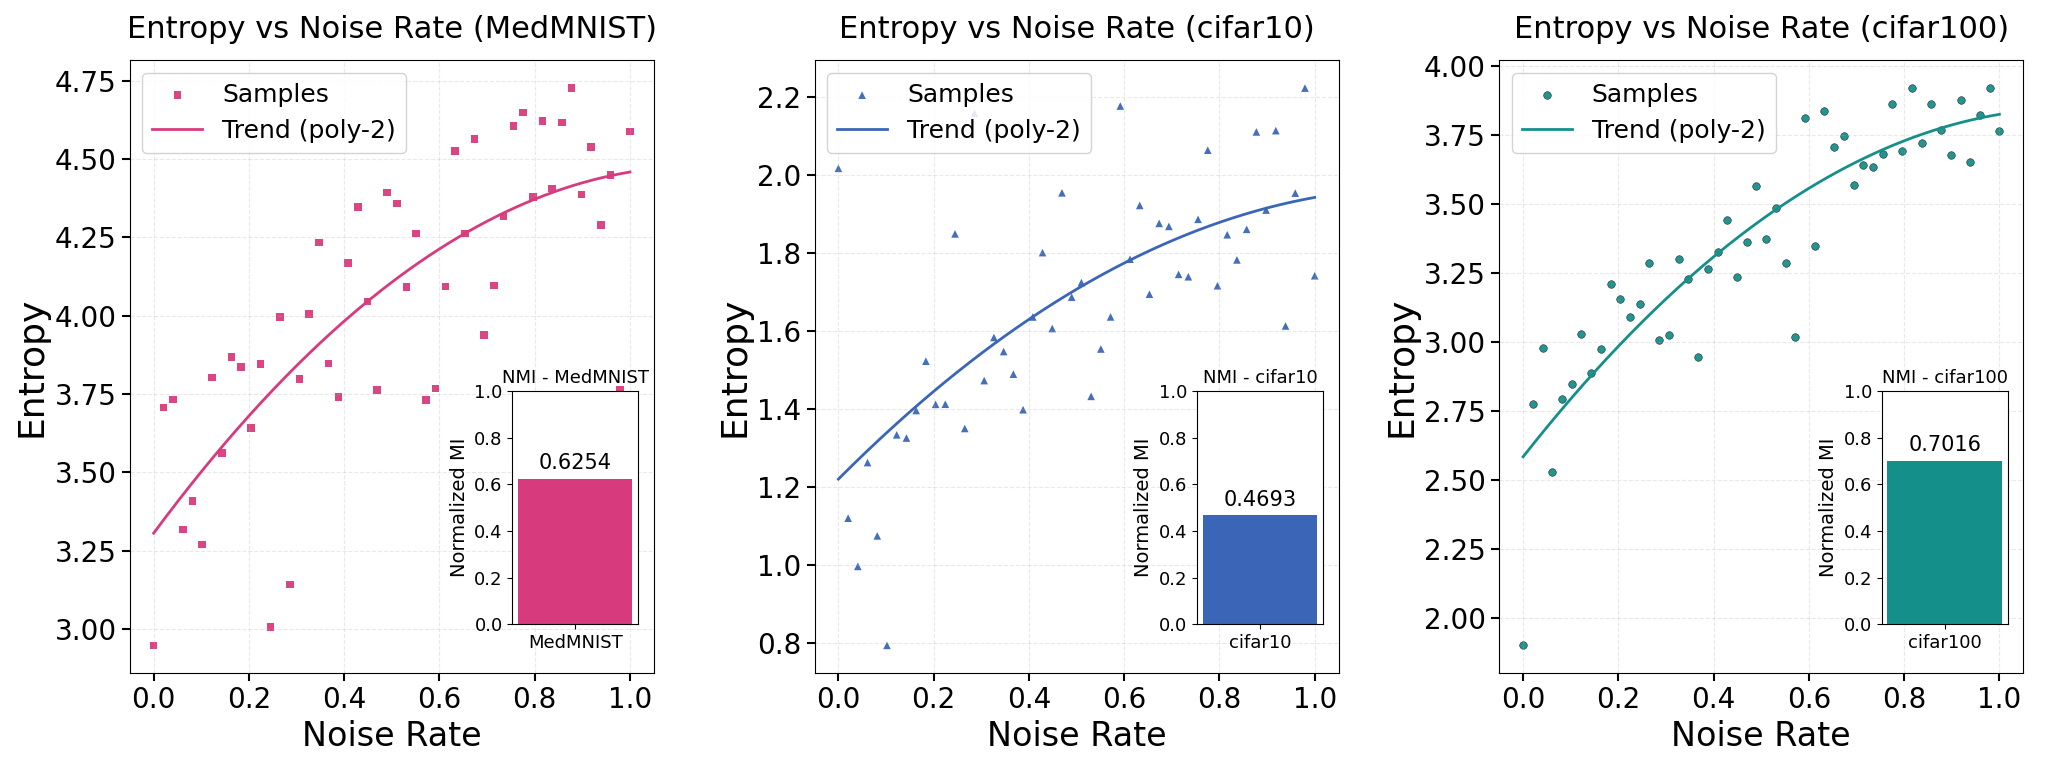
\includegraphics[width=\linewidth]{figure/entropy_noise_curve.png}
    \caption{Empirical relation between predictive entropy and client-side noise in our experiments. The curve shows that entropy increases as the noise level grows, supporting it as a lightweight reliability signal.}
    \label{fig:entropy}
\end{figure}

First, we use predictive entropy as a lightweight probing objective for client-block reliability. 
Figure~\ref{fig:entropy_illustration} illustrates the mechanism behind this probing.
After short local adaptation, each client model is evaluated on the same probing inputs at the server, and the entropy of its predictive distribution summarizes how concentrated or uncertain its probing-set predictions are.
A more formal bridge is provided in the supplementary material: under a standard symmetric label-noise transition model, and assuming the probing samples are sufficiently separable and the adapted client predictions are reasonably calibrated, the average predictive entropy is monotone increasing in the client noise rate up to a calibration- and separability-dependent relaxation.
This is consistent with classical noisy-label transition models~\cite{natarajan2013learning,patrini2017loss} and with confidence-based label diagnosis~\cite{northcutt2021confident,guo2017calibration}.
Consistent with this mechanism, Figure~\ref{fig:entropy} shows that predictive entropy is positively correlated with the client-side label noise rate in our experimental settings. 
Therefore, predictive entropy is used as an efficient probing-set reliability signal for identifying reliability outliers before training.
Its role is not to recover the true label-noise rate exactly, but to provide an observable ranking signal whose remaining mismatch is captured by the residual term below.

Let $\widetilde H_i\in[0,1]$ be the normalized predictive entropy of client $i$ on the probing set, and define the entropy-based set-level probing
\begin{equation}
\label{eq:entropy_probing_set}
\widehat{\xi}_{H}(S)
=
\sum_{i\in S}
\omega_i(S)\widetilde H_i,
\qquad
\omega_i(S)=\frac{n_i}{\sum_{j\in S}n_j}.
\end{equation}
Let $z_S$ be the probing-predicted class mixture of the retained client set, and let $p_{\mathrm{prob}}$ denote a target-facing reference prior used by the server. Here, \texttt{prob} is shorthand for probing.
In our implementation, $p_{\mathrm{prob}}$ is specified without using the true labels of the probing samples.
For numerical stability, define the smoothed mixture
\begin{equation}
\label{eq:smoothed_probing_mixture}
z_S^\epsilon
=
\frac{z_S+\epsilon \mathbf 1}{1+K\epsilon}.
\end{equation}

Rather than assuming that these proxies are exact, we define the following residual terms:
\begin{align}
\label{eq:entropy_residual}
r_H(S;c_H)
&=
\left[
\xi_{\mathrm{noise}}(S)
-
c_H\widehat{\xi}_{H}(S)
\right]_+,\\
\label{eq:coverage_residual}
r_Z(S)
&=
\frac12\|\bar q_S-z_S\|_1,\\
\label{eq:target_probing_residual}
r_T
&=
\frac12\|p_{\mathrm{prob}}-q_T\|_1,\\
\label{eq:smoothing_residual}
r_\epsilon(S)
&=
\frac12\|z_S-z_S^\epsilon\|_1,
\end{align}
where $[a]_+=\max\{a,0\}$ and $c_H>0$ is a scaling constant.
Here, $r_H$ measures the gap between the population noise-contamination term and the entropy-based probing, $r_Z$ measures the mismatch between the probing-predicted mixture and the clean selected-client prior, $r_T$ measures the mismatch between the server-side reference prior and the target prior, and $r_\epsilon$ accounts for smoothing.

\begin{theorem}[Residualized probing outlier-removal bound]
\label{thm:residualized_probing_bound}
Under Assumptions~\ref{assump:bounded_loss}--\ref{assump:label_only_noise}, for any selected subset $S$, any $h\in\mathcal H$, and any $c_H>0$,
\begin{equation}
	\label{eq:residualized_probing_bound}
	\begin{aligned}
		\epsilon_T(h)
		\le\;&
		\epsilon_S^n(h)
		+
		c_H\widehat{\xi}_{H}(S)
		+
		\sqrt{
			\frac12
			\mathrm{KL}
			\left(
			p_{\mathrm{prob}}\|z_S^\epsilon
			\right)
		}
		\\
		&+
		R_{\mathrm{prob}}(S;c_H).
	\end{aligned}
\end{equation}
where
\begin{equation}
\label{eq:probing_residual_total}
R_{\mathrm{prob}}(S;c_H)
=
r_H(S;c_H)
+
r_Z(S)
+
r_T
+
r_\epsilon(S).
\end{equation}
\end{theorem}

Theorem~\ref{thm:residualized_probing_bound} separates the observable part of the bound from the residual terms that quantify probing mismatch.
Thus, FedOCR optimizes the observable surrogate, while $R_{\mathrm{prob}}(S;c_H)$ captures the remaining gap between probing statistics and population quantities.

\begin{corollary}[probing-consistency outlier-removal surrogate]
\label{cor:probing_consistency_surrogate}
Suppose that the probing residual is uniformly bounded over the candidate subsets under consideration, i.e.,
$R_{\mathrm{prob}}(S;c_H)\le \delta_{\mathrm{prob}}$.
Then, for any $\lambda_s>0$,
\begin{equation}
\label{eq:probing_consistency_bound}
\epsilon_T(h)
\le
\epsilon_S^n(h)
+
c_H\widehat{\xi}_{H}(S)
+
\lambda_s
\mathrm{KL}
\left(
p_{\mathrm{prob}}\|z_S^\epsilon
\right)
+
\delta_{\mathrm{prob}}
+
\frac{1}{8\lambda_s}.
\end{equation}
\end{corollary}

Corollary~\ref{cor:probing_consistency_surrogate} motivates the computable subset-level outlier-removal surrogate
\begin{equation}
\label{eq:probing_surrogate_objective}
\widehat{\mathcal B}(S)
=
\lambda_m\widehat{\xi}_{H}(S)
+
\lambda_s
\mathrm{KL}
\left(
p_{\mathrm{prob}}\|z_S^\epsilon
\right),
\end{equation}
where $\lambda_m$ absorbs the unknown scaling constant $c_H$.
This surrogate is the observable part of the residualized probing bound.
The residual terms are not directly optimized by FedOCR; they characterize the approximation gap introduced by using probing statistics.
Accordingly, the theory provides a probing-consistency justification for FedOCR: the main risk bound specifies which population factors should be controlled, and the residualized bound states when the observable entropy--KL surrogate is aligned with those factors.
When the probing residuals are small, minimizing the surrogate controls the target-risk bound up to the residual gap.
Additional discussion of the residual terms is provided in the supplementary material.

\section{Method}
\label{sec:method}

The theoretical analysis motivates an additive probing objective consisting of an entropy-based predictive unreliability term and a probing distribution-mismatch term. 
FedOCR implements this objective through the following four components:
\begin{itemize}
	\item \textbf{probing instantiation.} We instantiate the theory-derived probing objective using normalized predictive entropy and probing-KL matching.
	\item \textbf{Client-block scoring.} We convert the additive objective into a local candidate-wise retention score for greedy client-block outlier removal.
	\item \textbf{Noise-adaptive calibration.} We optionally apply noise-adaptive exponents to calibrate the filtering strictness under heterogeneous noise.
	\item \textbf{Variable-size retention.} We use a variable-size prefix rule to determine how many clients should be retained.
\end{itemize}
Only the first two components are directly tied to the probing objective, while the adaptive exponent and prefix-threshold mechanisms are practical choices for improving robustness under heterogeneous noise.

\subsection{Reliability Surrogate via Fixed-Scale Predictive Entropy}
\label{subsec:reliability_surrogate}

Before outlier removal, each candidate client starts from the current global model and performs a short local adaptation, producing a client model $f_i$.
This adaptation is performed once before federated training, using a small fixed local budget $E_{\mathrm{adm}}$, and all candidate clients follow the same protocol.
Let $p_i(c\mid x)$ denote the predictive probability of client model $f_i$ on probing input $x\in\mathcal D_{\mathrm{prob}}$.
We define the average predictive entropy of client $i$ as
\begin{equation}
\label{eq:entropy_main}
H_i
=
-\frac{1}{|\mathcal D_{\mathrm{prob}}|}
\sum_{x\in\mathcal D_{\mathrm{prob}}}
\sum_{c=1}^{K}
p_i(c\mid x)\log p_i(c\mid x).
\end{equation}
For a $K$-class categorical distribution, the maximum entropy is $\log K$, achieved by the uniform distribution.
We therefore normalize $H_i$ as $\widetilde H_i=H_i/\log K$, so that $\widetilde H_i\in[0,1]$ in theory.
A value close to $1$ indicates near-uniform predictive uncertainty on the probing set, which we use as an observable probing for predictive unreliability.
In implementation, $\widetilde H_i$ is clipped to $[0,1]$ only for numerical stability.
The fixed-scale reliability score is
\begin{equation}
\label{eq:quality_score}
C_m(i)
=
\max\{1-\widetilde H_i,\epsilon\},
\end{equation}
where $\epsilon>0$ prevents zero reliability and keeps the negative-log cost finite.
At the set level, this score corresponds to the entropy-based probing term $\widehat{\xi}_{H}(S)=\sum_{i\in S}\omega_i(S)\widetilde H_i$, where $\omega_i(S)=n_i/\sum_{j\in S}n_j$.
Thus, retaining clients with larger $C_m(i)$ discourages the outlier-removal client set from accumulating high estimated predictive unreliability.

\subsection{Representativeness Surrogate via probing-Predicted Class Signatures}
\label{subsec:representativeness_surrogate}

Let $p_{\mathrm{prob}}\in\Delta^{K-1}$ be a server-side target reference prior.
For balanced benchmarks, we use the uniform class prior; in deployments, it can be provided by the expected target distribution.
FedOCR does not use the true labels of $\mathcal D_{\mathrm{prob}}$.
For each client $i$, we construct a probing-predicted class signature from hard predictions:
\begin{equation}
\label{eq:predictive_signature_main}
r_i(c)
=
\sum_{x\in\mathcal D_{\mathrm{prob}}}
\mathbf{1}
\left[
\arg\max_{c'}p_i(c'\mid x)=c
\right],
\qquad c=1,\dots,K.
\end{equation}
Let $\hat r_i=r_i/(\sum_{c=1}^{K}r_i(c)+\epsilon)$ denote the normalized signature.
For a selected subset $S$, we define the probing-predicted mixture as
\begin{equation}
\label{eq:subset_signature_main}
z_S
=
\sum_{i\in S}
\omega_i(S)\hat r_i
\in\Delta^{K-1},
\qquad
\omega_i(S)=\frac{n_i}{\sum_{j\in S}n_j}.
\end{equation}
In theory, we would like to know the true clean class distribution of the retained client set.
However, the server cannot observe each client's clean label prior $q_i$ in FL.
Therefore, FedOCR uses the observable prediction signature $\hat r_i$ on the probing set as a practical substitute.
The resulting mixture $z_S$ should not be viewed as an exact estimate of the clients' true clean label distribution.
Instead, it measures which target-relevant classes are covered by the retained client models on the probing set, reflecting the role of label-prior and distribution mismatch in Non-IID generalization~\cite{lipton2018labelshift,hsu2019measuring,zhu2021survey}.

For numerical stability, we apply $\epsilon$-smoothing before computing KL divergence:
\begin{equation}
	z_S^\epsilon=\frac{z_S+\epsilon\mathbf 1}{1+K\epsilon}.
\end{equation}
For a candidate client $k\notin S$, we measure the distribution mismatch after retaining $k$ by $d(k\mid S)=\mathrm{KL}(p_{\mathrm{prob}}\|z_{S\cup\{k\}}^\epsilon)$ and convert it into the distribution score
\begin{equation}
\label{eq:distribution_score}
C_s(k\mid S)
=
\exp\!\left(-\tau d(k\mid S)\right).
\end{equation}
We use the forward direction $\mathrm{KL}(p_{\mathrm{prob}}\|z_{S\cup\{k\}}^\epsilon)$ because missing reference target classes in the retained pool should be penalized strongly.
When $\tau$ is not fixed, we calibrate it from the valid candidate pool $\mathcal V$ by setting $\tau=(Q_{q_\tau}(\{d(i\mid\emptyset):i\in\mathcal V\})+\epsilon)^{-1}$.
This calibration makes the score less sensitive to the absolute KL scale of a particular dataset or candidate pool.

\subsection{From Additive Surrogate to Local Retention Score}
\label{subsec:local_retention_score}

The additive probing objective in Eq.~\eqref{eq:probing_surrogate_objective} is a set-level objective.
FedOCR does not solve this combinatorial problem exactly.
Instead, it greedily minimizes a local candidate-wise approximation, following the common use of greedy procedures in subset and client selection problems~\cite{nemhauser1978submodular,krause2014submodular,sener2018coreset,zhang2023dpp}.
For a candidate client $k\notin S$, the post-retention KL term $\mathrm{KL}(p_{\mathrm{prob}}\|z_{S\cup\{k\}}^\epsilon)$ measures the distribution mismatch after retaining $k$, while the entropy term $\widetilde H_k$ serves as a local approximation to the marginal increase of the set-level unreliability term.

A direct fixed-score implementation of the additive surrogate is
\begin{equation}
\label{eq:fixed_retention_score}
A_0(k\mid S)
=
\exp
\left(
-\lambda_s
\mathrm{KL}
\left(
p_{\mathrm{prob}}\|z_{S\cup\{k\}}^\epsilon
\right)
-
\lambda_m\widetilde H_k
\right).
\end{equation}
This score directly exponentiates the additive surrogate. Since the exponential
of a weighted sum factorizes into a product, Eq.~\eqref{eq:fixed_retention_score}
naturally motivates a multiplicative score over the two components. Using the
bounded monotone scores defined above, namely $C_s(k\mid S)$ in
Eq.~\eqref{eq:distribution_score} and $C_m(k)$ in Eq.~\eqref{eq:quality_score},
we obtain the practical retention utility
\begin{equation}
\label{eq:adaptive_utility}
A(k\mid S)
=
C_s(k\mid S)^{a_{\mathrm{eff}}}
C_m(k)^{b_{\mathrm{eff}}}.
\end{equation}
This form preserves the preference direction of the additive surrogate while
keeping both factors bounded and numerically stable. Fixed exponents give the
non-adaptive version, whereas adaptive exponents reweight the two components
during client-block outlier removal.


The multiplicative form is conservative: a client must be both distributionally useful and sufficiently reliable to obtain a high score.
Equivalently, maximizing $A(k\mid S)$ is minimizing the negative-log retention cost
\begin{align}
\label{eq:retention_cost}
R(k\mid S)
&=
-\log A(k\mid S)\\
&=
a_{\mathrm{eff}}\tau
\mathrm{KL}\!\left(p_{\mathrm{prob}}\|z_{S\cup\{k\}}^\epsilon\right)
+
b_{\mathrm{eff}}\big[-\log C_m(k)\big].
\end{align}
Eq.~\eqref{eq:retention_cost} can be viewed as a local candidate-wise negative-log approximation to Eq.~\eqref{eq:probing_surrogate_objective}, with $-\log C_m(k)$ replacing the marginal entropy cost and the forward KL measuring the post-retention distribution mismatch.
For small to moderate entropy values, $-\log(1-\widetilde H_k)\approx \widetilde H_k$, while highly uncertain clients receive a stronger penalty.

\subsection{Optional Noise-Adaptive Calibration}
\label{subsec:adaptive_calibration}

The adaptive exponents are practical calibration terms, not a direct consequence of the risk bound.
The core theory-aligned version uses fixed weights in Eq.~\eqref{eq:fixed_retention_score}.
However, a fixed reliability--representativeness trade-off can be suboptimal under heterogeneous noise.
When the candidate pool is severely noisy, outlier removal should emphasize reliability; when the pool is moderately noisy, representativeness becomes more important for target-distribution coverage~\cite{liang2023fednoisy,wu2023fednoro}.

We estimate the global predictive unreliability level from normalized entropy scores:
\begin{equation}
\label{eq:global_noise_score}
s
=
\rho\,\mathrm{Mean}(\{\widetilde H_i\}_{i\in\mathcal V})
+
(1-\rho)\,Q_q(\{\widetilde H_i\}_{i\in\mathcal V}),
\qquad
\rho\in[0,1].
\end{equation}
Given $s$, define $g=\mathrm{clip}(2(0.5-s),-1,1)$.
Let $a$ and $b$ be base exponents.
We use $a_{\mathrm{eff}}=\mathrm{clip}(a(1+\lambda g),a_{\min},a_{\max})$ and $\bar b_{\mathrm{eff}}=\mathrm{clip}(b(1-\lambda g),b_{\min},b_{\max})$.
For datasets with many classes, entropy is harder to calibrate; hence we use the class-scaled exponent $b_{\mathrm{eff}}=\bar b_{\mathrm{eff}}(\max\{K/K_b,1\})^{-\nu_b}$, where $K_b$ is a reference class number and $\nu_b\ge0$ controls the scaling strength.
When $s>0.5$, $g<0$, so $a_{\mathrm{eff}}$ decreases and $b_{\mathrm{eff}}$ increases; the outlier-removal rule emphasizes reliability under severe uncertainty.
When $s<0.5$, the rule increases the distribution weight and encourages broader target-distribution coverage.
We evaluate the fixed-score variant and the adaptive variant separately in the ablation study.

\subsection{Variable-Size Greedy Outlier-Removal Set Construction}
\label{subsec:variable_greedy}

\begin{algorithm}[t]
\caption{FedOCR: Fixed-Scale Noise-Adaptive Client-Block Outlier Removal}
\label{alg:FedOCR}
\begin{algorithmic}[1]
\Require Candidate clients $[N]$, sample sizes $\{n_i\}_{i=1}^N$, probing set $\mathcal D_{\mathrm{prob}}$, outlier-removal adaptation budget $E_{\mathrm{adm}}$, greedy horizon $M$, minimum retained budget $K_{\min}$, parameters $\rho,q,a,b,\lambda,\tau,q_\tau,\eta_{\min},\eta_{\max},\tau_K$
\Ensure Outlier-removal client set $S^\star$
\State $\mathcal V\leftarrow[N]$, $S_0\leftarrow\emptyset$, $J(S_0)\leftarrow0$
\For{$i\in\mathcal V$}
    \State Obtain client model $f_i$ after short local adaptation with budget $E_{\mathrm{adm}}$
    \State Compute predictive entropy $H_i$ by Eq.~\eqref{eq:entropy_main}
    \State Normalize entropy as $\widetilde H_i\leftarrow H_i/\log K$
    \State Compute reliability score $C_m(i)$ by Eq.~\eqref{eq:quality_score}
    \State Compute probing-predicted signature $r_i$ by Eq.~\eqref{eq:predictive_signature_main}
\EndFor
\State Set label-free target reference prior $p_{\mathrm{prob}}$
\State Compute global unreliability score $s$ by Eq.~\eqref{eq:global_noise_score}
\State Compute $a_{\mathrm{eff}}$ and $b_{\mathrm{eff}}$ as described in Section~\ref{subsec:adaptive_calibration}
\State Calibrate $\tau$ if not fixed, and compute adaptive benchmark $\eta(s,K;\tau_K)$ by Eq.~\eqref{eq:eta_temp}
\For{$m=1,\dots,\min(M,|\mathcal V|)$}
    \For{each $k\in\mathcal V\setminus S_{m-1}$}
        \State Form smoothed mixture $z_{S_{m-1}\cup\{k\}}^\epsilon$
        \State Compute $C_s(k\mid S_{m-1})$ by Eq.~\eqref{eq:distribution_score}
        \State Compute $A(k\mid S_{m-1})$ by Eq.~\eqref{eq:adaptive_utility}
    \EndFor
    \State $k_m\leftarrow\arg\max_{k\in\mathcal V\setminus S_{m-1}}A(k\mid S_{m-1})$
    \State $S_m\leftarrow S_{m-1}\cup\{k_m\}$
    \State $J(S_m)\leftarrow J(S_{m-1})+\log\frac{A(k_m\mid S_{m-1})}{\eta(s,K;\tau_K)}$
\EndFor
\State $S^\star\leftarrow \arg\max_{S_m:\,m\ge K_{\min}}J(S_m)$
\State \Return $S^\star$
\end{algorithmic}
\end{algorithm}

Many existing client selection methods assume a predefined per-round participation budget, such as a fixed fraction or a fixed number of clients
\cite{mcmahan2017communication, lai2021oort, cho2022power}.
FedOCR instead lets the final participant pool size be determined by the greedy outlier-removal sequence, and uses a temperature coefficient to regulate the retained cardinality.

We use the full candidate pool $\mathcal V=[N]$.
FedOCR then constructs a greedy sequence $S_1\subset S_2\subset\cdots\subset S_M$, where $M$ is the greedy horizon.
At step $m$, the retained client is
\begin{equation}
\label{eq:greedy_step}
k_m
=
\arg\max_{k\in\mathcal V\setminus S_{m-1}}
A(k\mid S_{m-1}),
\qquad
S_m=S_{m-1}\cup\{k_m\}.
\end{equation}

The KL-based objective is not generally submodular, so the greedy rule should be viewed as a practical approximation rather than an approximation-guaranteed optimizer~\cite{nemhauser1978submodular,krause2014submodular}.
Its role is to construct a high-scoring retention sequence, from which the final pool size is selected by a noise-adaptive prefix objective.

To decide how many clients to retain after outlier removal, we use a noise-adaptive benchmark with a cardinality temperature coefficient $\tau_K>0$.
Given the global unreliability score $s$, define
\[
\eta_0(s)=\mathrm{clip}(\eta_{\min}+(\eta_{\max}-\eta_{\min})s,\epsilon,1),
\]
and
\begin{equation}
\label{eq:eta_temp}
\eta(s,K;\tau_K)
=
\mathrm{clip}\!\left(
\left[
\eta_0(s)\bigl(\max\{K/K_\eta,1\}\bigr)^{-\nu_\eta}
\right]^{\tau_K},
\epsilon,1
\right).
\end{equation}
A larger $s$ yields a stricter baseline; $\tau_K$ controls the selection aggressiveness.
Because the inner benchmark lies in $(0,1]$, larger $\tau_K$ decreases the effective retention threshold and tends to retain more clients, while smaller $\tau_K$ yields a more conservative pool.

For each prefix $S_m$, we compute the cumulative threshold-normalized objective
\begin{equation}
\label{eq:prefix_objective}
J(S_m)
=
\sum_{t=1}^{m}
\log
\frac{
A(k_t\mid S_{t-1})
}{
\eta(s,K;\tau_K)
}.
\end{equation}
Equivalently,
\[
J(S_m)=\sum_{t=1}^{m}\log A(k_t\mid S_{t-1})-m\log\eta(s,K;\tau_K),
\]
which is an accumulated retention utility with a noise-adaptive cardinality penalty.
Under a minimum client constraint $K_{\min}$, the final outlier-removal client set is
\begin{equation}
\label{eq:variable_size_selection}
S^\star
=
\arg\max_{S_m:\,m\ge K_{\min}}
J(S_m).
\end{equation}
This mechanism adapts the retained client count to the observed quality and distributional complementarity of the candidate pool.
In high-uncertainty regimes, the retained set can shrink to avoid unreliable clients; when the candidate pool is mostly reliable and complementary, the method can retain more useful clients.

% \paragraph{Complexity.}
% FedOCR introduces a one-time pre-training screening cost.
% Scoring candidates requires $O(|\mathcal V|E_{\mathrm{adm}})$ local adaptation cost, where $E_{\mathrm{adm}}$ is the short outlier-removal adaptation budget.
% probing evaluation requires $O(|\mathcal V||\mathcal D_{\mathrm{prob}}|)$ forward passes.
% After probing signatures are computed, each greedy step evaluates at most $|\mathcal V|$ candidates with $K$-dimensional class mixtures, giving $O(M|\mathcal V|K)$ scoring cost for a greedy horizon $M$.
% These costs are incurred once before federated optimization, rather than at every communication round.


Algorithm~\ref{alg:FedOCR} summarizes the complete FedOCR procedure.

\begin{table*}[!t]
	\centering
	\caption{\normalfont Test accuracy (\%) of representative noisy-label FL and client-selection methods under heterogeneous label noise on MedMNIST~\cite{yang2023medmnist}, CIFAR-10~\cite{krizhevsky2009learning}, and CIFAR-100~\cite{krizhevsky2009learning}. Results are collected at $\alpha=0.5$ with 50 candidate clients and reported as mean$\pm$standard deviation. FedOCR uses the proposed automatic client-block outlier-removal rule in this table. Best results are highlighted in bold and second-best results are underlined.}
	\label{tab:noisy_fl_accuracy}
	\setlength{\tabcolsep}{3.2pt}
	\renewcommand{\arraystretch}{1.15}
	\begin{tabular}{lcccccc}
		\toprule
		\multirow{2}{*}{\textbf{Method}} 
		& \multicolumn{2}{c}{\textbf{MedMNIST}} 
		& \multicolumn{2}{c}{\textbf{CIFAR-10}} 
		& \multicolumn{2}{c}{\textbf{CIFAR-100}} \\
		\cmidrule(lr){2-3} \cmidrule(lr){4-5} \cmidrule(lr){6-7}
		& \textbf{Linear} & \textbf{Gaussian} & \textbf{Linear} & \textbf{Gaussian} & \textbf{Linear} & \textbf{Gaussian} \\
		\midrule
		
		All & 60.89$\pm$1.89 & 85.53$\pm$0.73 & 39.16$\pm$0.31 & 54.38$\pm$0.37 & 24.11$\pm$0.13 & 31.21$\pm$0.23 \\
		\midrule
		\multicolumn{7}{l}{\textit{Full-round robust training baselines}} \\
		RFA~\cite{pillutla2022robust} & 63.38$\pm$3.24 & 83.05$\pm$0.67 & 35.52$\pm$0.10 & 47.68$\pm$0.45 & 20.52$\pm$0.07 & 30.31$\pm$0.23 \\
		FedGreed~\cite{kritharakis2025fedgreed} & 83.09$\pm$3.17 & 82.22$\pm$3.67 & 55.05$\pm$0.85 & 54.24$\pm$1.68 & 20.79$\pm$1.05 & 32.18$\pm$0.86 \\
		LASA~\cite{xu2025lasa} & 54.97$\pm$0.51 & 87.52$\pm$0.57 & 42.97$\pm$0.23 & 56.20$\pm$0.31 & 23.69$\pm$0.15 & 31.03$\pm$0.12 \\
		FedNed~\cite{lu2024fedned} & 64.29$\pm$0.54 & 86.52$\pm$0.58 & 39.72$\pm$0.09 & 55.41$\pm$0.30 & 23.63$\pm$0.04 & 32.73$\pm$0.11 \\
		FedNoRo~\cite{wu2023fednoro} & \underline{85.48$\pm$0.41} & 87.22$\pm$0.42 & 51.14$\pm$0.21 & \underline{61.09$\pm$0.34} & 28.56$\pm$0.09 & 33.28$\pm$0.16 \\
		\midrule
		\multicolumn{7}{l}{\textit{Training-stage correction baselines}} \\
		FedCorr~\cite{xu2022fedcorr} & 55.54$\pm$13.10 & 85.18$\pm$1.02 & 53.39$\pm$0.33 & 49.59$\pm$0.77 & 26.19$\pm$0.17 & 30.67$\pm$0.28 \\
		FedCS~\cite{hao2025fedcs} & 56.60$\pm$3.02 & 79.12$\pm$0.76 & 31.77$\pm$0.48 & 47.43$\pm$0.25 & 19.84$\pm$0.33 & 23.46$\pm$0.18 \\
		FedFixer~\cite{ji2024fedfixer} & 61.06$\pm$1.92 & 85.70$\pm$0.76 & 33.53$\pm$0.39 & 54.61$\pm$0.42 & 23.45$\pm$0.17 & 32.71$\pm$0.25 \\
		FedDiv~\cite{li2024feddiv} & 60.75$\pm$1.91 & 85.39$\pm$0.75 & 41.84$\pm$0.74 & 54.49$\pm$0.16 & 22.53$\pm$0.51 & 31.40$\pm$0.12 \\
		\midrule
		\multicolumn{7}{l}{\textit{Client-selection baselines}} \\
		PoC~\cite{cho2022power} & 54.34$\pm$2.75 & 79.68$\pm$2.12 & 14.79$\pm$0.29 & 44.58$\pm$0.65 & 25.46$\pm$0.21 & 30.05$\pm$0.25 \\
		GS~\cite{ma2021client} & 65.50$\pm$3.71 & 82.97$\pm$0.90 & 46.88$\pm$0.45 & 42.43$\pm$0.73 & 26.95$\pm$0.14 & 23.60$\pm$0.23 \\
		FedCor~\cite{tang2022fedcor} & 70.43$\pm$3.77 & 86.15$\pm$1.32 & 38.22$\pm$2.06 & 52.17$\pm$0.58 & 26.60$\pm$0.16 & 33.41$\pm$0.11 \\
		\midrule
		FedOCR (ours) & 81.05$\pm$0.20 & 85.71$\pm$0.37 & \underline{56.60$\pm$0.24} & 58.68$\pm$0.41 & 28.73$\pm$0.35 & 33.63$\pm$0.34 \\
		FedOCR + FedCor~\cite{tang2022fedcor} & 67.82$\pm$5.69 & 82.12$\pm$0.29 & 56.09$\pm$0.18 & 60.62$\pm$0.46 & $\boldsymbol{30.94\pm0.23}$ & 32.28$\pm$0.17 \\
		FedOCR + FedCorr~\cite{xu2022fedcorr} & 79.73$\pm$2.15 & \underline{88.89$\pm$1.11} & $\boldsymbol{57.01\pm0.84}$ & 53.07$\pm$0.78 & 28.70$\pm$0.28 & \underline{34.94$\pm$0.33} \\
		FedOCR + FedNoRo~\cite{wu2023fednoro} & $\boldsymbol{86.19\pm0.41}$ & $\boldsymbol{91.32\pm0.39}$ & 55.68$\pm$0.36 & $\boldsymbol{67.89\pm0.35}$ & \underline{30.27$\pm$0.16} & $\boldsymbol{35.49\pm0.13}$ \\
		\bottomrule
	\end{tabular}
\end{table*}

\section{Experiments}
\label{sec:experiment}
In this section, we first use a controlled oracle experiment to check whether the theoretical bound matches empirical target risk. We then evaluate FedOCR on three benchmark datasets under heterogeneous label noise and Non-IID settings, and we examine its robustness, cost, probing-set sensitivity, retained-pool composition, and ablation behavior.
\subsection{Oracle Experiment}
\label{subsec:oracle_exp}
We consider a three-class Gaussian classification problem with two-dimensional features, class-balanced target prior, and six candidate clients that differ in both label prior and symmetric label-noise rate(shown in table\ref{tab:oracle_setup}).
The purpose of this experiment is not to benchmark practical methods, but to check whether the risk factors in Theorem~\ref{thm:main_bound} rank retained client-block sets in the expected order.
The four retention strategies isolate the effects of no outlier removal, distribution mismatch, label noise, and the oracle FedOCR-style admission rule.
\begin{table}[t]
	\centering
    \caption{\normalfont Configuration of the oracle experiment. The six clients differ in both class-prior distribution and label-noise rate. Clients C1--C3 are low-noise but individually class-skewed, while their union provides a balanced class distribution.}
	\label{tab:oracle_setup}
	\setlength{\tabcolsep}{4pt}
	\renewcommand{\arraystretch}{1.15}
	\begin{tabular}{l|l}
		\toprule
		\textbf{Item} & \textbf{Setting} \\
		\midrule
		Task type & Three-class non-IID classification \\
		Feature dimension & 2 \\
		Input distribution & Gaussian class-conditionals \\
		Class means & $\mu_1=(-2,0),\ \mu_2=(2,0),\ \mu_3=(0,2)$ \\
		Covariance & $\sigma=0.9$ \\
		Target prior & $q_T=(1/3,1/3,1/3)$ \\
		Label noise & Symmetric noise with rate $\rho$ \\
		Noise mechanism & Flip to other $K-1$ classes uniformly \\
		Model & Two-layer MLP, $2 \rightarrow 16 \rightarrow 3$ \\
		Activation & ReLU \\
		Optimizer & Full-batch gradient descent \\
		Learning rate & $0.01$ \\
		Training epochs & 400 epochs, including epoch 0 initialization \\
		Initialization & $\mathcal{N}(0,0.01)$ with fixed random seed \\
		Samples per client & 300 \\
		Target test set & 3000 clean samples with balanced class prior \\
		\bottomrule
	\end{tabular}
\end{table}
Figure~\ref{fig:oracle_risk} compares the empirical target risk and the dynamic theoretical upper bound under four oracle retention strategies.
\begin{figure}[t]
	\centering
	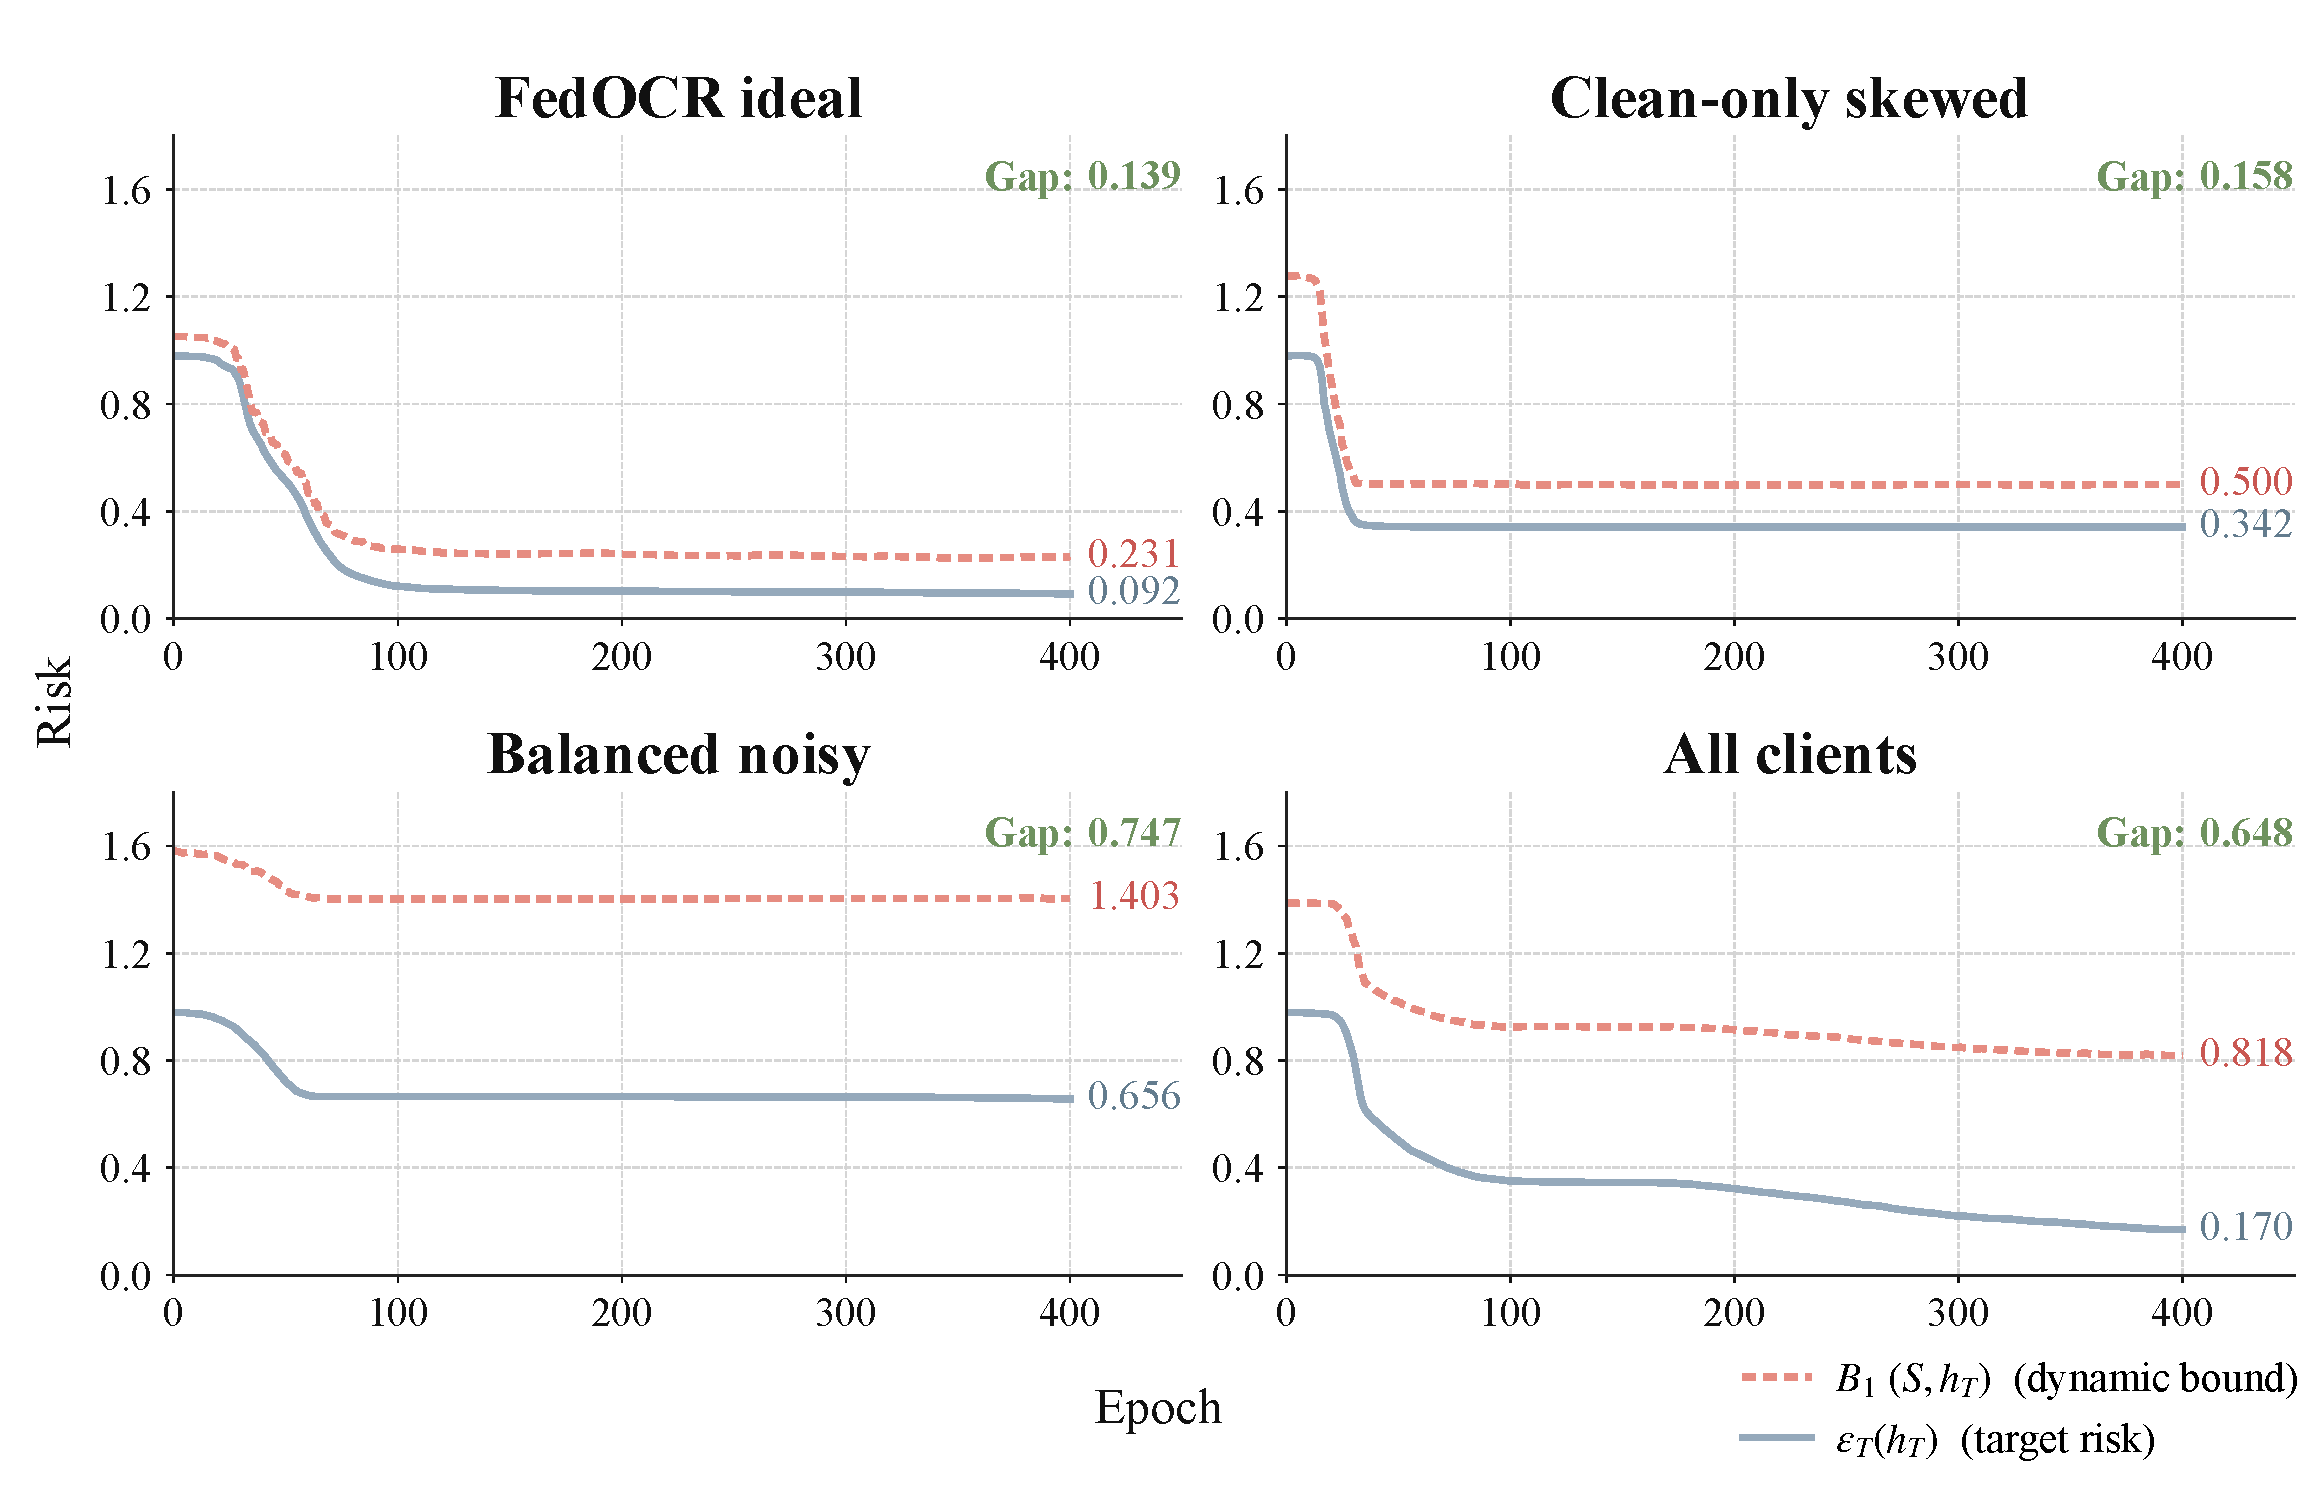
\includegraphics[width=\linewidth]{figure/oracle/risk_bound.pdf}
	\caption{Empirical target risk and theoretical upper bound during oracle training.}
	\label{fig:oracle_risk}
\end{figure}
The most informative pattern is not that one strategy merely gets a lower final number, but that the bound tracks the same ordering as the empirical risk throughout training.
The FedOCR ideal strategy, which retains $C1$, $C2$, and $C3$, drives both curves down fastest because it removes the noisiest client while still preserving the class coverage that the target task needs.
The clean-only skewed pool $(C1,C2)$ shows the opposite failure mode: removing the worst noise source helps, but the retained pool is still too narrow, so the risk does not fall as far.
The balanced-noisy singleton $C4$ keeps class coverage but leaves the supervision too corrupted to support low risk.
Using all clients sits between these extremes because it mixes noisy and mismatched clients in one pool.
So the oracle plot does more than rank strategies; it confirms that the theoretical bound captures the same cleanliness-versus-coverage tension that drives the empirical target risk.
The bound view tells the same story from another angle.
Figure~\ref{fig:oracle_bound} shows that the FedOCR ideal strategy has the tightest bound, the noisy but balanced singleton has the loosest one, and the all-client pool again falls in between.
This means the theory is not just abstract: it ranks the oracle retained sets in the same order as the measured target risk.
\begin{figure}[t]
    \centering
    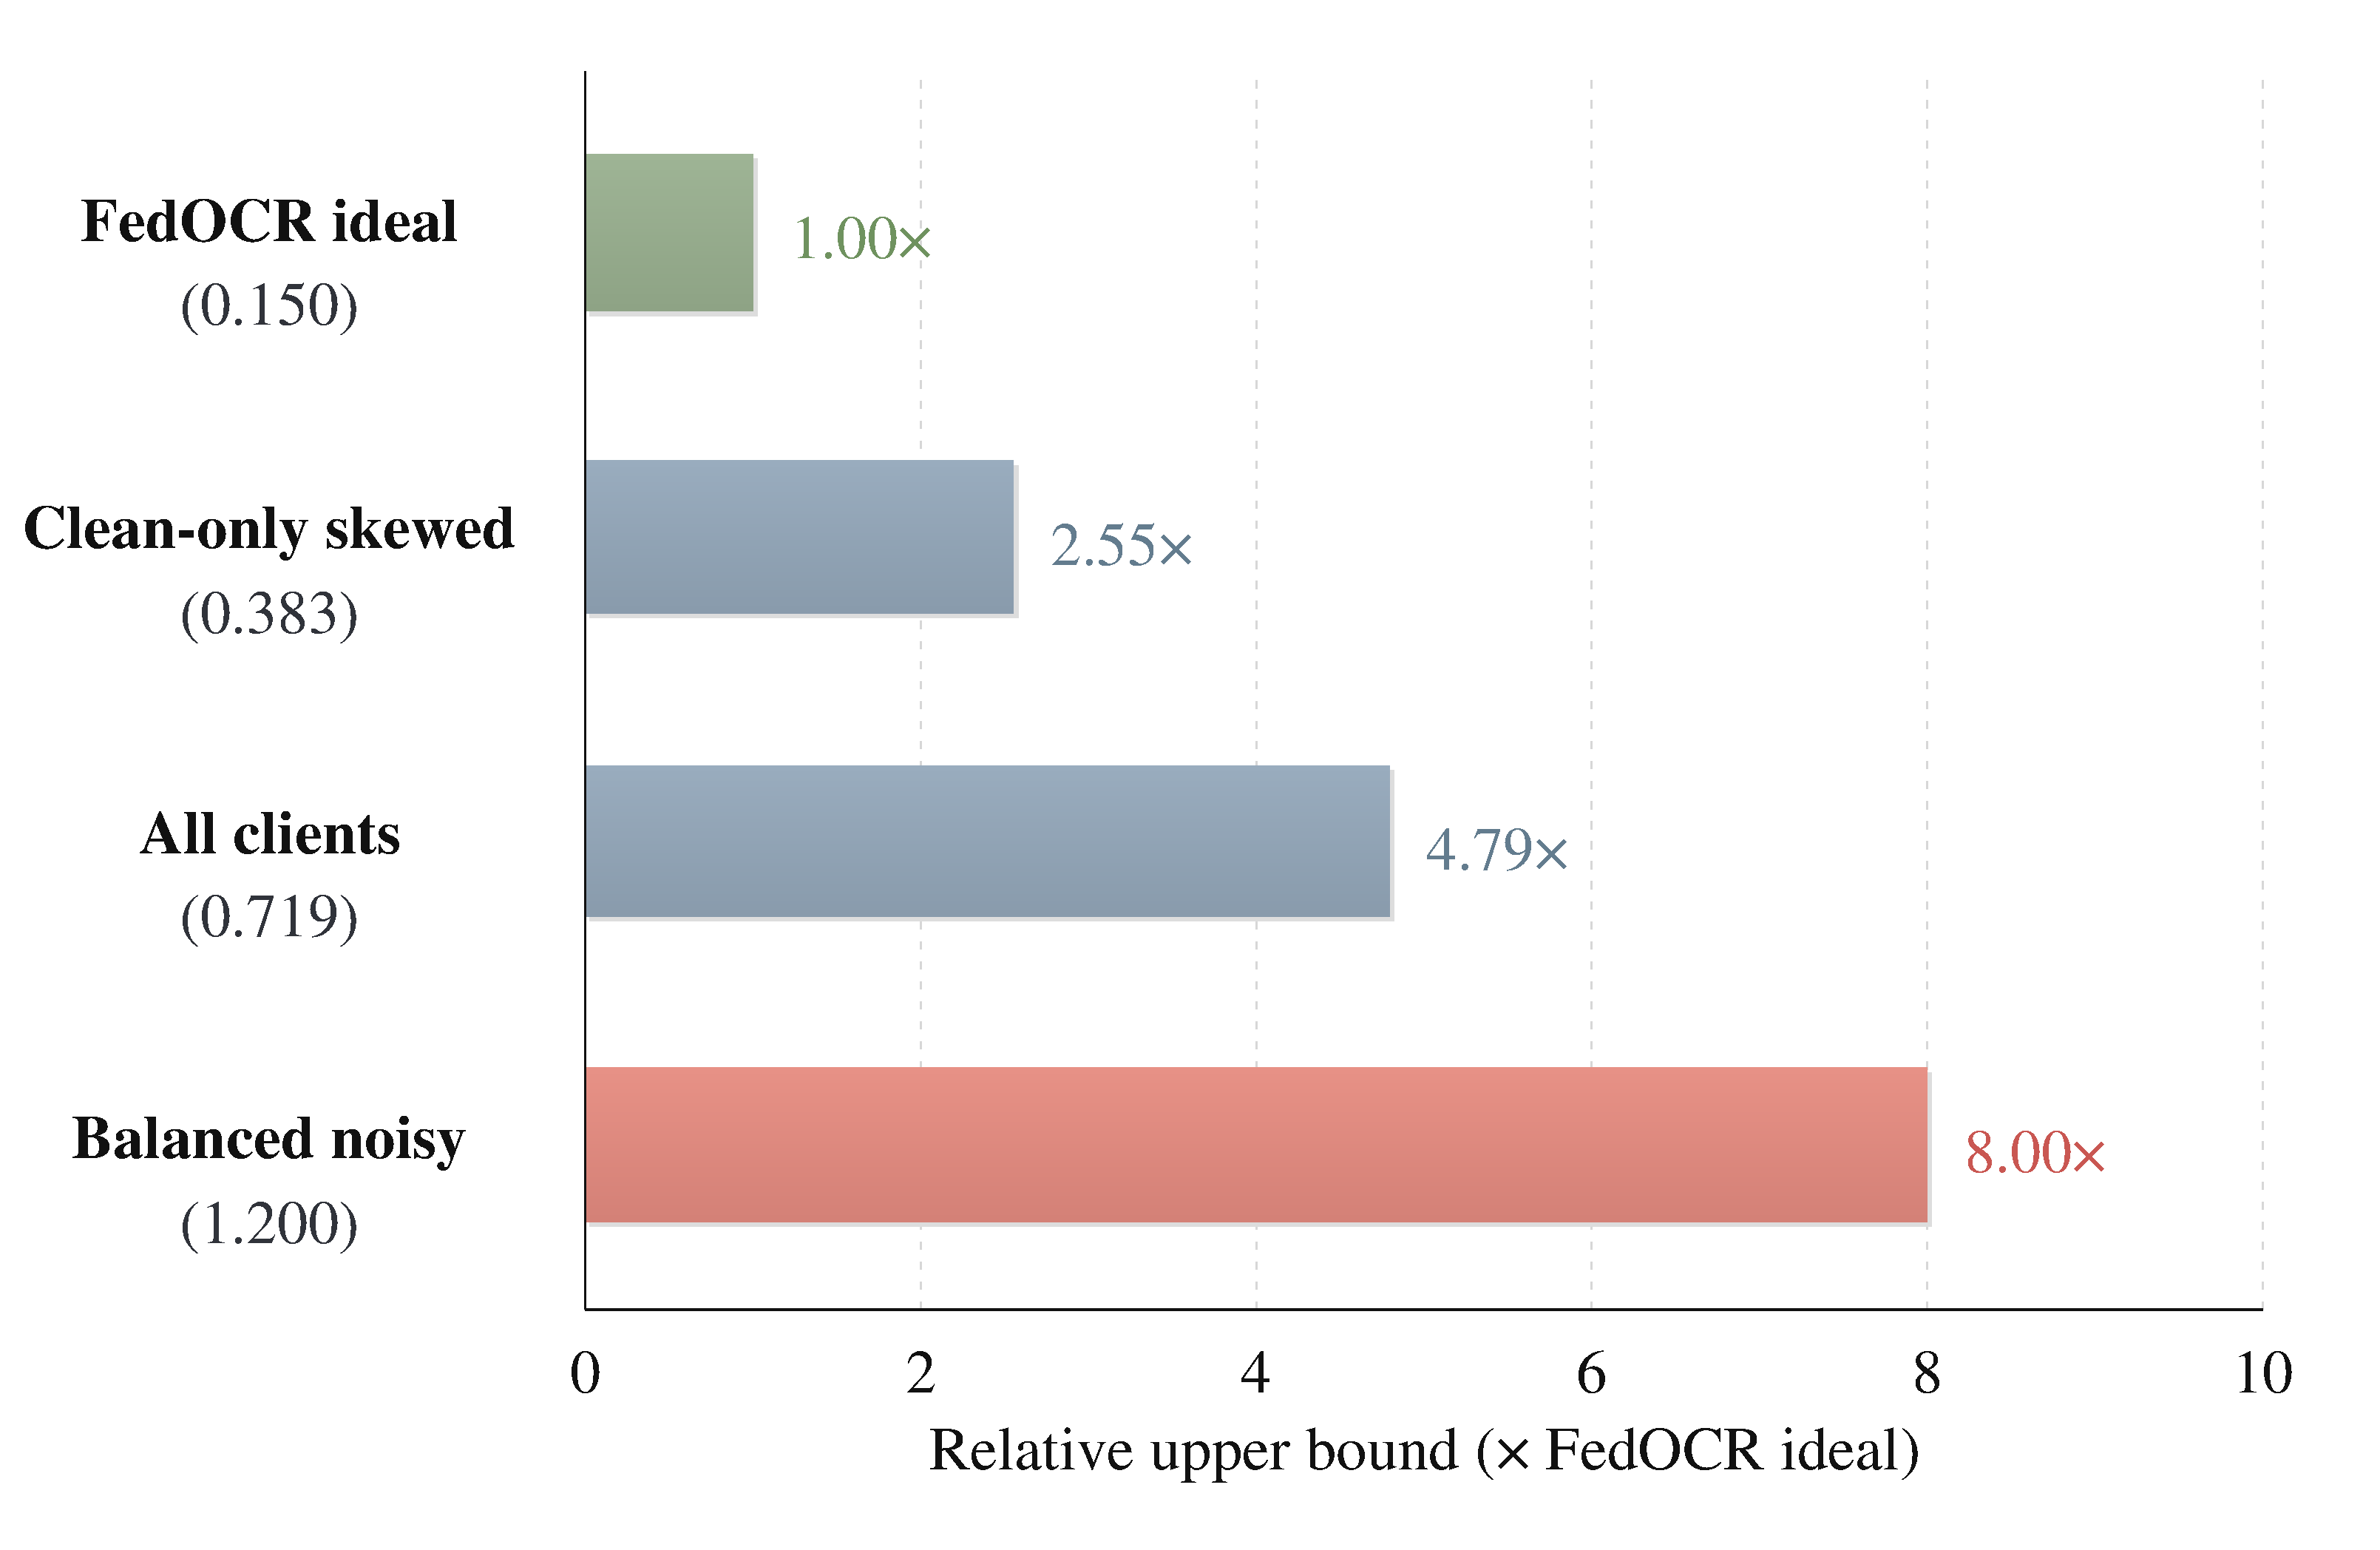
\includegraphics[width=0.92\linewidth]{figure/oracle/theoretical_bound.pdf}
    \caption{\normalfont Theoretical risk bound under different oracle retention strategies.}
    \label{fig:oracle_bound}
\end{figure}
\begin{table*}[!t]
	\centering
	\caption{\normalfont Cost comparison at matched target accuracy. For each scenario, the reference method is selected as a representative strong baseline from the three baseline families considered in Table~\ref{tab:noisy_fl_accuracy}, including full-round robust training baselines, training-stage correction baselines, and client-selection baselines. Computation is reported in $10^6$ FEP and communication in GB. Saving denotes the computation / communication reduction of FedOCR-based methods relative to the corresponding reference method. Negative values indicate higher cost than the reference method. Best and second-best costs within each scenario are highlighted in bold and underlined, respectively.}
	\label{tab:efficiency_linear}
	\setlength{\tabcolsep}{4.5pt}
	\renewcommand{\arraystretch}{1.12}
	\begin{tabular}{llcccc}
		\toprule
		\textbf{Scenario} & \textbf{Method} & \textbf{Target} & \textbf{Comp.} & \textbf{Comm.} & \textbf{Saving} \\
		\midrule
		\multirow{3}{*}{MedMNIST Linear} 
		& FedNoRo & \multirow{3}{*}{80\%} & 2.62 & 41.66 & -- \\
		& FedOCR (ours) & & \underline{1.04} & $\boldsymbol{14.66}$ & \underline{60.3\%} / $\boldsymbol{64.8\%}$ \\
		& FedOCR (ours) + FedNoRo & & $\boldsymbol{0.84}$ & \underline{18.50} & $\boldsymbol{67.9\%}$ / \underline{55.6\%} \\
		\midrule
		
		\multirow{3}{*}{MedMNIST Gaussian} 
		& FedNoRo & \multirow{3}{*}{85\%} & 3.21 & 54.16 & -- \\
		& FedOCR (ours) & & $\boldsymbol{1.78}$ & $\boldsymbol{26.16}$ & $\boldsymbol{44.5\%}$ / $\boldsymbol{51.7\%}$ \\
		& FedOCR (ours) + FedNoRo & & \underline{2.15} & \underline{35.49} & \underline{33.0\%} / \underline{34.5\%} \\
		\midrule
		
		\multirow{3}{*}{CIFAR-10 Linear} 
		& FedCorr & \multirow{3}{*}{50\%} & 13.16 & 49.16 & -- \\
		& FedOCR (ours) & & $\boldsymbol{3.08}$ & $\boldsymbol{11.17}$ & $\boldsymbol{76.6\%}$ / $\boldsymbol{77.3\%}$ \\
		& FedOCR (ours) + FedCor & & \underline{3.72} & \underline{20.75} & \underline{71.7\%} / \underline{57.8\%} \\
		\midrule
		
		\multirow{3}{*}{CIFAR-10 Gaussian} 
		& FedCorr & \multirow{3}{*}{50\%} & \underline{7.08} & \underline{34.25} & -- \\
		& FedOCR (ours) & & $\boldsymbol{4.47}$ & $\boldsymbol{18.33}$ & $\boldsymbol{36.9\%}$ / $\boldsymbol{46.5\%}$ \\
		& FedOCR (ours) + FedCor & & 7.37 & 54.24 & -4.1\% / -58.4\% \\
		\midrule
		
		\multirow{3}{*}{CIFAR-100 Linear} 
		& FedCorr & \multirow{3}{*}{28\%} & \underline{13.14} & 85.30 & -- \\
		& FedOCR (ours) & & $\boldsymbol{9.84}$ & $\boldsymbol{71.81}$ & $\boldsymbol{25.1\%}$ / $\boldsymbol{15.8\%}$ \\
		& FedOCR (ours) + FedCorr & & 16.78 & \underline{72.26} & -27.7\% / \underline{15.3\%} \\
		\midrule
		
		\multirow{3}{*}{CIFAR-100 Gaussian} 
		& FedCorr & \multirow{3}{*}{30\%} & 11.67 & 45.18 & -- \\
		& FedOCR (ours) & & $\boldsymbol{8.12}$ & \underline{44.76} & $\boldsymbol{30.4\%}$ / \underline{0.9\%} \\
		& FedOCR (ours) + FedCorr & & \underline{9.03} & $\boldsymbol{41.89}$ & \underline{22.6\%} / $\boldsymbol{7.3\%}$ \\
		\bottomrule
	\end{tabular}
\end{table*}

\subsection{Main experiments}
\label{subsec:exp_setup}
In this section, we first present a controlled oracle experiment to validate our theoretical analysis. We then evaluate FedOCR on three benchmark datasets under heterogeneous label-noise and Non-IID settings, comparing it with representative noisy-label FL and client-selection baselines, and further studying its efficiency, sensitivity, and ablation behavior.	
\paragraph{\textbf{Experimental setup}}
We evaluate FedOCR on MedMNIST~\cite{yang2023medmnist} and CIFAR-10/100~\cite{krizhevsky2009learning}. 
Unless otherwise specified, the training data are distributed over $N=50$ clients, and $K=20$ clients are selected for each federated training run. 
We simulate Non-IID data using Dirichlet partitioning with concentration parameter $\alpha=0.5$ and a step-imbalance ratio of 5~\cite{hsu2019measuring,li2021silos,zhu2021survey}. 
Client-level symmetric label noise is then injected following standard noisy-label robustness protocols~\cite{natarajan2013learning,patrini2017loss,liang2023fednoisy}. 
We consider two heterogeneous noise modes: \textit{linear noise}, where client noise rates are evenly spaced in $[0,1]$, and \textit{Gaussian noise}, where rates are drawn from $\mathcal{N}(0.3,0.15^2)$ and clipped to $[0,1]$. 
The former provides a controllable high-noise stress test, while the latter models a more random corruption pattern closer to practical uncertainty.

All methods are trained under the same maximum budget of $T=200$ global rounds. 
For FedOCR's admission stage, we use a short 10-epoch local adaptation to compute the filtering indicators, keeping the pre-screening lightweight and consistent with the deployment-oriented design. 
For local training, all methods use Adam with learning rate $1\times10^{-4}$ and batch size 64.

We compare against three baseline families:
\begin{itemize}
	\setlength{\itemsep}{0.1em}
	\setlength{\topsep}{0.15em}
	\setlength{\parsep}{0pt}
	\item \textbf{Full-round robust training baselines:} RFA~\cite{pillutla2022robust}, FedGreed~\cite{kritharakis2025fedgreed}, LASA~\cite{xu2025lasa}, FedNed~\cite{lu2024fedned}, and FedNoRo~\cite{wu2023fednoro}.
	\item \textbf{Training-stage correction baselines:} FedCorr~\cite{xu2022fedcorr}, FedCS~\cite{hao2025fedcs}, FedFixer~\cite{ji2024fedfixer}, and FedDiv~\cite{li2024feddiv}.
	\item \textbf{Client-selection baselines:} All, RS, EMD, GS~\cite{ma2021client}, PoC~\cite{cho2022power}, and FedCor~\cite{tang2022fedcor}.
\end{itemize}

\paragraph{\textbf{Comparison with baselines}}
\label{para:comp_nfl}
We first compare FedOCR with noisy-label FL baselines under linear and Gaussian heterogeneous noise to evaluate noisy-label robustness.
Table~\ref{tab:noisy_fl_accuracy} reports the accuracy results on MedMNIST~\cite{yang2023medmnist}, CIFAR-10~\cite{krizhevsky2009learning}, and CIFAR-100~\cite{krizhevsky2009learning}.
Unless otherwise stated, every standalone FedOCR entry in our tables and figures denotes \textbf{FedOCR+FedAvg}; we omit ``+FedAvg'' for brevity because FedAvg is the default downstream optimizer after the admission stage.
The table also includes representative client-selection baselines under the same noise settings.
The four FedOCR rows separate the admission effect from downstream adaptation: the standalone row applies the proposed pre-training client-block outlier-removal rule and then runs standard FedAvg, while the other rows place the same rule before FedCor, FedCorr, or FedNoRo.

Two patterns stand out. First, standalone FedOCR improves all six dataset-noise settings over full participation, and the largest gains appear under linear noise. This means the admission stage removes the client blocks that do the most damage before their updates spread through training.
Second, the combination rows show that FedOCR is a front-end module, not a universal fix. FedOCR+FedNoRo is best in the four settings where a robust downstream learner can use the cleaner pool most effectively, while FedOCR+FedCorr and FedOCR+FedCor win in the two linear cases where the remaining corruption is better matched by correction.
So the table supports a simple conclusion: admission gives the main robustness gain, and downstream correction is only a regime-specific add-on.

Table~\ref{tab:efficiency_linear} isolates the system-level picture at matched target accuracy.
For each scenario, the reference baseline is a strong non-FedOCR method from Table~\ref{tab:noisy_fl_accuracy} that reaches the target.
The message is simple: admission is where most wasted work disappears.
FedOCR alone reaches the target with the lowest cost in most scenarios because it removes high-risk clients before they consume communication and local epochs.
When a downstream correction method is attached, the result becomes a trade-off between extra overhead and better recovery of residual noise.
So the table says that the pre-training filter is the main cost saver, and downstream correction helps only when its gain is worth the extra cost.
In practice, this means we should not expect every FedOCR-plus-correction combination to be cost-effective; if the downstream method brings only a small accuracy gain, the extra communication and local computation can outweigh the benefit.

We also test whether the conclusion changes with the strength of Non-IID partitioning.
Table~\ref{tab:noniid_robustness} reports the CIFAR-10 results under linear noise for $\alpha\in\{0.1,0.5,1.0\}$.
The trend is clear. FedOCR is strongest at the two ends of the range and stays near the top in the middle.
That means client-block filtering helps most when skew and corruption are both strong.
When heterogeneity is milder, methods that keep more clients can close the gap.

\begin{table}[h]
\centering
\caption{\normalfont CIFAR-10 accuracy (\%) under linear noise with different Dirichlet Non-IID levels. Results are reported as mean$\pm$standard deviation. Best results are highlighted in bold and second-best results are underlined.}
\label{tab:noniid_robustness}
\setlength{\tabcolsep}{5pt}
\renewcommand{\arraystretch}{1.10}
\begin{tabular}{lccc}
\toprule
\textbf{Method} & $\alpha=0.1$ & $\alpha=0.5$ & $\alpha=1.0$ \\
\midrule
All & 26.22$\pm$0.21 & 39.16$\pm$0.31 & 49.10$\pm$0.41 \\
RFA~\cite{pillutla2022robust} & 23.88$\pm$0.34 & 35.52$\pm$0.10 & 40.95$\pm$0.28 \\
FedGreed~\cite{kritharakis2025fedgreed} & 23.55$\pm$1.98 & \underline{55.05$\pm$0.85} & 55.75$\pm$1.52 \\
LASA~\cite{xu2025lasa} & 26.68$\pm$0.28 & 42.97$\pm$0.23 & 45.57$\pm$0.53 \\
FedNed~\cite{lu2024fedned} & 26.01$\pm$0.36 & 39.72$\pm$0.09 & 49.75$\pm$0.32 \\
FedNoRo~\cite{wu2023fednoro} & \underline{29.80$\pm$0.41} & 51.31$\pm$0.42 & \underline{56.53$\pm$0.20} \\
FedCorr~\cite{xu2022fedcorr} & 25.29$\pm$1.43 & 53.35$\pm$0.33 & 44.93$\pm$0.50 \\
FedCS~\cite{hao2025fedcs} & 20.52$\pm$0.37 & 31.77$\pm$0.48 & 35.21$\pm$1.47 \\
FedFixer~\cite{ji2024fedfixer} & 26.78$\pm$0.21 & 33.53$\pm$0.39 & 48.89$\pm$0.41 \\
FedDiv~\cite{li2024feddiv} & 26.47$\pm$0.20 & 41.84$\pm$0.74 & 49.00$\pm$0.38 \\
\midrule
FedOCR (ours) & $\boldsymbol{30.27\pm0.35}$ & $\boldsymbol{56.60\pm0.24}$ & $\boldsymbol{57.48\pm0.37}$ \\
\bottomrule
\end{tabular}
\end{table}
\paragraph{\textbf{Hyperparameter sensitivity}}
We study three key hyperparameters in the outlier-removal stage: the noise-adaptive strength, the first-round local epoch budget used to compute filtering indicators, and the threshold range $\eta$.
Figure~\ref{fig:hyperparameter_sensitivity} reports the sensitivity results on the CIFAR-10 linear-noise setting.
The figure shows a real trade-off.
Too little filtering leaves noisy clients in the pool.
Too much filtering removes useful coverage.
FedOCR works best in the middle, which is what we want from an admission rule.

\begin{figure}[t]
    \centering
    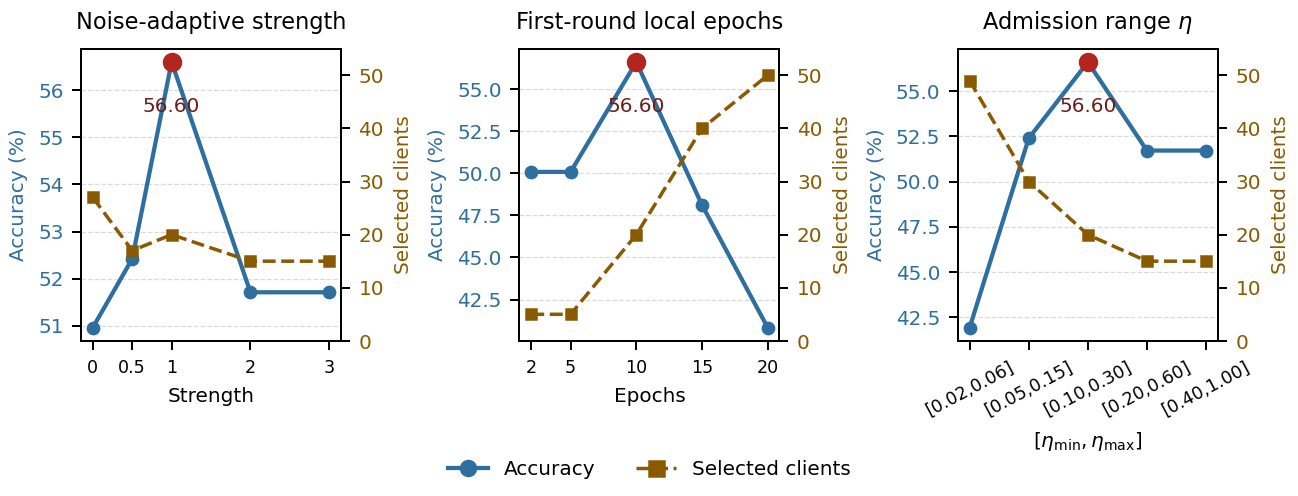
\includegraphics[width=\linewidth]{figure/hyperparameter_sensitivity.png}
    \caption{Hyperparameter sensitivity on CIFAR-10 under linear heterogeneous noise. Each panel reports the test accuracy and the number of retained clients when varying one outlier-removal-stage hyperparameter while keeping the others fixed.}
    \label{fig:hyperparameter_sensitivity}
\end{figure}

For the strength coefficient, the best result is obtained at strength $=1$; smaller values keep too many risky clients, while larger values over-prune the pool.
For the first-round epoch budget, 10 epochs give the most useful filtering indicators: too few epochs produce weak entropy estimates, while too many epochs make even risky clients look too confident on the probing set and shrink the gap between good and bad clients.
For $\eta$, the default range $[0.10,0.30]$ selects 20 clients and achieves the best accuracy; smaller ranges keep too many noisy clients, while larger ranges are too strict.
Additional client-pool-size curves are provided in the supplementary material.

\paragraph{\textbf{Probing-set sensitivity}}
This table asks one question: how hard is it to build a probing set for FedOCR?
Table~\ref{tab:probing_set_sensitivity} reports probing-set configurations on CIFAR-10~\cite{krizhevsky2009learning} under the same linear-noise setting used in the dedicated probe study (\emph{ResNet18}, $\alpha=0.5$, and $\eta\in[0.1,0.3]$).
All runs use a fixed random seed, so identical rows mean that FedOCR selected the same client set and followed the same training trajectory.
The size sweep gives the main answer: even a 1\% probing set, or 100 images in total, stays very close to the best result.
So FedOCR does not need a large clean probe, which keeps the collection cost low.
The Dirichlet sweep shows a smaller effect: mild input-distribution changes perturb accuracy only slightly, so the probe does not need to be perfectly IID.
The label-noise sweep is flat because FedOCR never uses probing labels.
That means label quality is not a real requirement here, which makes the probing set much easier to build in practice.
\begin{table}[!t]
	\centering
	\caption{\normalfont FedOCR probing-set sensitivity on CIFAR-10~\cite{krizhevsky2009learning} under linear heterogeneous noise. Results are reported as the last five rounds' mean$\pm$standard deviation, together with the final retained client count and the number of sample scans used by the admission stage.}
	\label{tab:probing_set_sensitivity}
	\setlength{\tabcolsep}{3.6pt}
	\renewcommand{\arraystretch}{1.12}
	\scriptsize
	\begin{tabular}{llccc}
		\toprule
		\textbf{Family} & \textbf{Setting} & \textbf{Acc. (\%)} & \textbf{Retained} & \textbf{Sample scans} \\
		\midrule
		\multirow{7}{*}{Size}
		& 1\%   & 56.77$\pm$0.44 & 14 & 100 \\
		& 2\%   & 56.82$\pm$0.43 & 14 & 200 \\
		& 5\%   & $\boldsymbol{57.10\pm0.33}$ & 15 & 500 \\
		& 10\%(default)  & 56.60$\pm$0.24 & 15 & 1000 \\
		& 20\%  & 55.04$\pm$0.34 & 14 & 2000 \\
		& 50\%  & 55.07$\pm$0.45 & 14 & 5000 \\
		& 100\% & 54.58$\pm$0.78 & 14 & 9000 \\
		\midrule
		\multirow{5}{*}{Dirichlet}
		& $IID$(default) & $\boldsymbol{56.60\pm0.24}$ & 15 & 1000 \\
		& $\alpha=10$ & 55.88$\pm$0.39 & 15 & 1000 \\
		& $\alpha=1$  & 55.85$\pm$0.59 & 13 & 1000 \\
		& $\alpha=0.5$ & 55.25$\pm$0.38 & 8 & 1000 \\
		& $\alpha=0.1$ & 56.04$\pm$0.34 & 11 & 1000 \\
		\midrule
		\multirow{5}{*}{Noise}
		& clean(default) & 56.60$\pm$0.24 & 15 & 1000 \\
		& 10\% & 56.60$\pm$0.24 & 15 & 1000 \\
		& 20\% & 56.60$\pm$0.24 & 15 & 1000 \\
		& 30\% & 56.60$\pm$0.24 & 15 & 1000 \\
		& 50\%& 56.60$\pm$0.24 & 15 & 1000 \\
		\bottomrule
	\end{tabular}
\end{table}


\subsection{Analysis of Selected Client Subsets}
\label{subsec:subset_analysis}

To understand why FedOCR improves robustness, we analyze the class-wise sample mass and noise rate of the retained client sets.
Figure~\ref{fig:subset_composition_main} shows the retained pools under linear heterogeneous noise.
FedOCR keeps the cleanest pool among the compared methods and still spreads mass across classes.
RS and Fixed keep broader pools, but they also keep more noisy mass.
EMD, PoC, and GS do not solve this trade-off either: they can improve coverage, but they still retain many noisy classes.
So the figure says the same thing as the accuracy table: FedOCR keeps clients that are both cleaner and more balanced.

\begin{figure}[t]
    \centering
    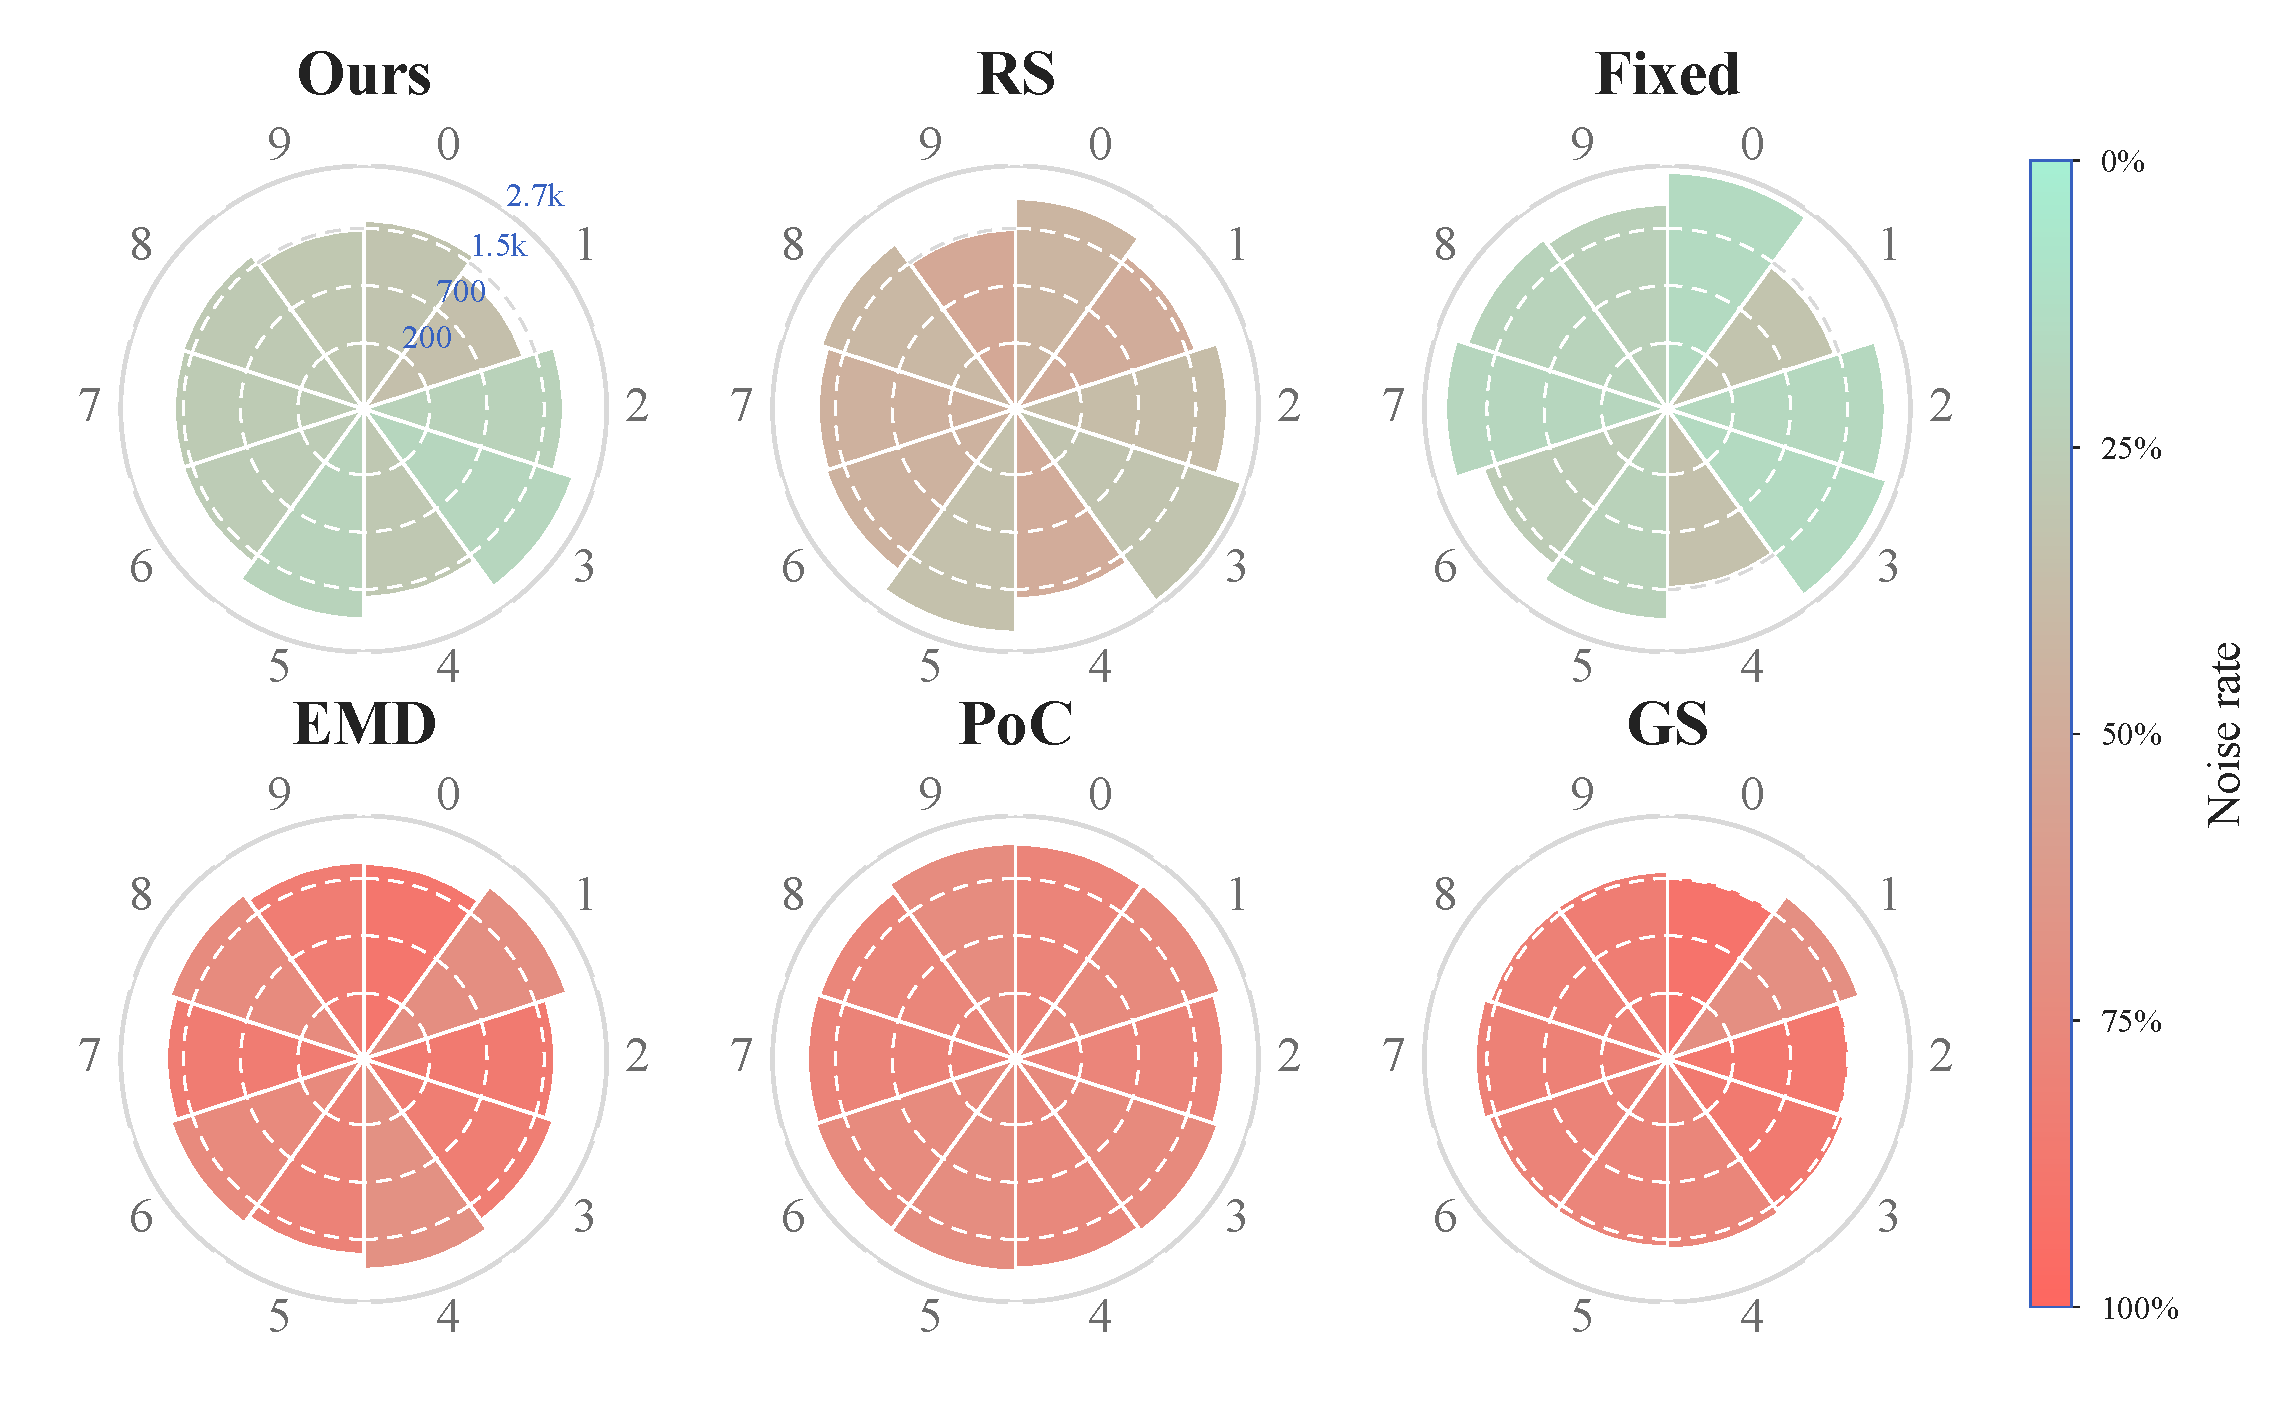
\includegraphics[width=\linewidth]{figure/data_distribution_fig9.pdf}
    \caption{\normalfont Class-wise sample-mass and noise-rate profile of the retained client sets under linear heterogeneous noise. The polar radius shows the retained sample mass, and the color encodes the class-wise noise rate from low (green) to high (red).}
    \label{fig:subset_composition_main}
\end{figure}




\subsection{Ablation Study}
\label{subsec:ablation}

We ablate the two scoring terms and the adaptive calibration mechanism.
Table~\ref{tab:ablation_fedraa} clarifies the role hierarchy inside FedOCR.
Reliability filtering is the main driver.
Once high-risk clients are removed, the retained pool is much easier to optimize, even without any representativeness term.
Representativeness alone cannot rescue a noisy pool, so the distribution-only variant still performs poorly.
Adaptive calibration adds a smaller but consistent gain by avoiding a fixed reliability-versus-coverage balance across all regimes.
So the components play different roles: reliability is the gatekeeper, representativeness protects coverage, and calibration adjusts the balance.

\begin{table}[h]
	\centering
	\caption{\normalfont Ablation study on CIFAR-10 under linear heterogeneous noise. The table isolates the effect of reliability scoring, representativeness scoring, and noise-adaptive calibration.}
	\label{tab:ablation_fedraa}
	\setlength{\tabcolsep}{2pt}
	\renewcommand{\arraystretch}{1.15}
	\begin{tabular}{lcccc}
		\toprule
		\textbf{Variant} 
		& \textbf{Reliab.} 
		& \textbf{Represent.} 
		& \textbf{Adaptive} 
		& \textbf{Test Acc. (\%)} \\
		\midrule
		
		Random selection     & -- & -- & -- & 39.81$\pm$0.32 \\
		All clients          & -- & -- & -- & 39.67$\pm$0.33 \\
		Reliability only     & \checkmark & $\times$ & $\times$ & \underline{54.60$\pm$0.30} \\
		Represent. only      & $\times$ & \checkmark & $\times$ & 30.69$\pm$0.52 \\
		w/o adaptive calib.  & \checkmark & \checkmark & $\times$ & 53.22$\pm$0.16 \\
		\midrule
		FedOCR               & \checkmark & \checkmark & \checkmark & $\boldsymbol{56.60\pm0.25}$ \\
		
		\bottomrule
	\end{tabular}
\end{table}
\section{Discussion}

FedOCR is a pre-training admission module: it removes risky client blocks before federated optimization starts, and the experiments show that this simple step improves robustness and reduces cost. The current version still has three clear limits.

\textbf{Theory scope.} Our theory assumes label-shift-dominated heterogeneity, where clients mainly differ in class priors (Assumption~\ref{assump:label_shift}). This keeps the analysis tractable, but it also means the guarantee is conditional rather than universal. When feature shift or domain shift is strong, predictive entropy and KL matching become weaker proxies~\cite{northcutt2021confident,guo2017calibration,ben2010theory,lipton2018labelshift}.

\textbf{Probe dependence.} FedOCR relies on a clean server-held probing set~\cite{mcmahan2017communication,kairouz2021advances}. The set does not need to be large, but it does need to be roughly target-relevant and refreshed when the deployment domain drifts. So FedOCR is robust to moderate probing mismatch, not arbitrary mismatch.

\textbf{Privacy boundary.} FedOCR is privacy-compatible, but it is not a formal privacy-preserving protocol. Although the probing set itself does not expose client data, server-client interaction may still leak coarse distributional information. A malicious server could, in principle, craft probing samples to infer whether a client contains certain classes or patterns. Stronger privacy defenses, such as differentially private entropy estimation, probe sanitization, encrypted probing, and secure evaluation, are left for future work.

Future work will also study more robust probing construction under domain shift, online updates for changing client populations, and when downstream correction is worth the extra communication and computation cost.

\section{Conclusion}

This paper studies robust federated learning by removing risky client blocks before training starts.
FedOCR builds an outlier-removal client set using two signals: probing-set predictive entropy for reliability and KL-based probing matching for representativeness.
Our theory explains why these two signals are related to label noise and target mismatch.

The experiments show three clear results.
First, FedOCR improves robustness under noisy and Non-IID settings.
Second, it reduces computation and communication cost at matched accuracy.
Third, it works with downstream noisy-label correction instead of replacing it.
Overall, FedOCR shows that robust FL can benefit from filtering bad clients early, not only from correcting updates during training.
Future work will study better probing construction, privacy-preserving probing, and online updates for long-running deployments~\cite{kairouz2021advances,fu2023client}.

\section*{Acknowledgments}
The authors acknowledge the use of ChatGPT for language polishing and wording refinement. The authors take full responsibility for the content, correctness, and originality of the manuscript.

\bibliographystyle{IEEEtran}
\bibliography{FedPeD_refs}


\end{document}
